% Options for packages loaded elsewhere
\PassOptionsToPackage{unicode}{hyperref}
\PassOptionsToPackage{hyphens}{url}
%
\documentclass[
]{article}
\usepackage{amsmath,amssymb}
\usepackage{iftex}
\ifPDFTeX
  \usepackage[T1]{fontenc}
  \usepackage[utf8]{inputenc}
  \usepackage{textcomp} % provide euro and other symbols
\else % if luatex or xetex
  \usepackage{unicode-math} % this also loads fontspec
  \defaultfontfeatures{Scale=MatchLowercase}
  \defaultfontfeatures[\rmfamily]{Ligatures=TeX,Scale=1}
\fi
\usepackage{lmodern}
\ifPDFTeX\else
  % xetex/luatex font selection
\fi
% Use upquote if available, for straight quotes in verbatim environments
\IfFileExists{upquote.sty}{\usepackage{upquote}}{}
\IfFileExists{microtype.sty}{% use microtype if available
  \usepackage[]{microtype}
  \UseMicrotypeSet[protrusion]{basicmath} % disable protrusion for tt fonts
}{}
\makeatletter
\@ifundefined{KOMAClassName}{% if non-KOMA class
  \IfFileExists{parskip.sty}{%
    \usepackage{parskip}
  }{% else
    \setlength{\parindent}{0pt}
    \setlength{\parskip}{6pt plus 2pt minus 1pt}}
}{% if KOMA class
  \KOMAoptions{parskip=half}}
\makeatother
\usepackage{xcolor}
\usepackage[margin=1in]{geometry}
\usepackage{color}
\usepackage{fancyvrb}
\newcommand{\VerbBar}{|}
\newcommand{\VERB}{\Verb[commandchars=\\\{\}]}
\DefineVerbatimEnvironment{Highlighting}{Verbatim}{commandchars=\\\{\}}
% Add ',fontsize=\small' for more characters per line
\usepackage{framed}
\definecolor{shadecolor}{RGB}{248,248,248}
\newenvironment{Shaded}{\begin{snugshade}}{\end{snugshade}}
\newcommand{\AlertTok}[1]{\textcolor[rgb]{0.94,0.16,0.16}{#1}}
\newcommand{\AnnotationTok}[1]{\textcolor[rgb]{0.56,0.35,0.01}{\textbf{\textit{#1}}}}
\newcommand{\AttributeTok}[1]{\textcolor[rgb]{0.13,0.29,0.53}{#1}}
\newcommand{\BaseNTok}[1]{\textcolor[rgb]{0.00,0.00,0.81}{#1}}
\newcommand{\BuiltInTok}[1]{#1}
\newcommand{\CharTok}[1]{\textcolor[rgb]{0.31,0.60,0.02}{#1}}
\newcommand{\CommentTok}[1]{\textcolor[rgb]{0.56,0.35,0.01}{\textit{#1}}}
\newcommand{\CommentVarTok}[1]{\textcolor[rgb]{0.56,0.35,0.01}{\textbf{\textit{#1}}}}
\newcommand{\ConstantTok}[1]{\textcolor[rgb]{0.56,0.35,0.01}{#1}}
\newcommand{\ControlFlowTok}[1]{\textcolor[rgb]{0.13,0.29,0.53}{\textbf{#1}}}
\newcommand{\DataTypeTok}[1]{\textcolor[rgb]{0.13,0.29,0.53}{#1}}
\newcommand{\DecValTok}[1]{\textcolor[rgb]{0.00,0.00,0.81}{#1}}
\newcommand{\DocumentationTok}[1]{\textcolor[rgb]{0.56,0.35,0.01}{\textbf{\textit{#1}}}}
\newcommand{\ErrorTok}[1]{\textcolor[rgb]{0.64,0.00,0.00}{\textbf{#1}}}
\newcommand{\ExtensionTok}[1]{#1}
\newcommand{\FloatTok}[1]{\textcolor[rgb]{0.00,0.00,0.81}{#1}}
\newcommand{\FunctionTok}[1]{\textcolor[rgb]{0.13,0.29,0.53}{\textbf{#1}}}
\newcommand{\ImportTok}[1]{#1}
\newcommand{\InformationTok}[1]{\textcolor[rgb]{0.56,0.35,0.01}{\textbf{\textit{#1}}}}
\newcommand{\KeywordTok}[1]{\textcolor[rgb]{0.13,0.29,0.53}{\textbf{#1}}}
\newcommand{\NormalTok}[1]{#1}
\newcommand{\OperatorTok}[1]{\textcolor[rgb]{0.81,0.36,0.00}{\textbf{#1}}}
\newcommand{\OtherTok}[1]{\textcolor[rgb]{0.56,0.35,0.01}{#1}}
\newcommand{\PreprocessorTok}[1]{\textcolor[rgb]{0.56,0.35,0.01}{\textit{#1}}}
\newcommand{\RegionMarkerTok}[1]{#1}
\newcommand{\SpecialCharTok}[1]{\textcolor[rgb]{0.81,0.36,0.00}{\textbf{#1}}}
\newcommand{\SpecialStringTok}[1]{\textcolor[rgb]{0.31,0.60,0.02}{#1}}
\newcommand{\StringTok}[1]{\textcolor[rgb]{0.31,0.60,0.02}{#1}}
\newcommand{\VariableTok}[1]{\textcolor[rgb]{0.00,0.00,0.00}{#1}}
\newcommand{\VerbatimStringTok}[1]{\textcolor[rgb]{0.31,0.60,0.02}{#1}}
\newcommand{\WarningTok}[1]{\textcolor[rgb]{0.56,0.35,0.01}{\textbf{\textit{#1}}}}
\usepackage{graphicx}
\makeatletter
\def\maxwidth{\ifdim\Gin@nat@width>\linewidth\linewidth\else\Gin@nat@width\fi}
\def\maxheight{\ifdim\Gin@nat@height>\textheight\textheight\else\Gin@nat@height\fi}
\makeatother
% Scale images if necessary, so that they will not overflow the page
% margins by default, and it is still possible to overwrite the defaults
% using explicit options in \includegraphics[width, height, ...]{}
\setkeys{Gin}{width=\maxwidth,height=\maxheight,keepaspectratio}
% Set default figure placement to htbp
\makeatletter
\def\fps@figure{htbp}
\makeatother
\setlength{\emergencystretch}{3em} % prevent overfull lines
\providecommand{\tightlist}{%
  \setlength{\itemsep}{0pt}\setlength{\parskip}{0pt}}
\setcounter{secnumdepth}{-\maxdimen} % remove section numbering
\ifLuaTeX
  \usepackage{selnolig}  % disable illegal ligatures
\fi
\IfFileExists{bookmark.sty}{\usepackage{bookmark}}{\usepackage{hyperref}}
\IfFileExists{xurl.sty}{\usepackage{xurl}}{} % add URL line breaks if available
\urlstyle{same}
\hypersetup{
  pdftitle={Lab 1 Report},
  pdfauthor={Marijn Jaarsma \& Simon Jorstedt \& Hugo Morvan},
  hidelinks,
  pdfcreator={LaTeX via pandoc}}

\title{Lab 1 Report}
\author{Marijn Jaarsma \& Simon Jorstedt \& Hugo Morvan}
\date{2023-11-19}

\begin{document}
\maketitle

\hypertarget{libraries}{%
\section{Libraries}\label{libraries}}

\begin{verbatim}
## Loading required package: ggplot2
\end{verbatim}

\begin{verbatim}
## Loading required package: lattice
\end{verbatim}

\hypertarget{assignment-1}{%
\section{Assignment 1}\label{assignment-1}}

\hypertarget{section}{%
\subsection{1.1}\label{section}}

\begin{quote}
Import the data into R and divide it into training, validation and test
sets (50\%/25\%/25\%) by using the partitioning principle specified in
the lecture slides.
\end{quote}

\begin{Shaded}
\begin{Highlighting}[]
\CommentTok{\# Read data}
\NormalTok{digit\_data }\OtherTok{\textless{}{-}} \FunctionTok{read.csv}\NormalTok{(}\StringTok{"optdigits.csv"}\NormalTok{, }\AttributeTok{header=}\ConstantTok{FALSE}\NormalTok{)}

\CommentTok{\# Partition data (according to Oleg)}
\NormalTok{n }\OtherTok{=} \FunctionTok{dim}\NormalTok{(digit\_data)[}\DecValTok{1}\NormalTok{]}

\FunctionTok{set.seed}\NormalTok{(}\DecValTok{12345}\NormalTok{)}
\NormalTok{id }\OtherTok{=} \FunctionTok{sample}\NormalTok{(}\DecValTok{1}\SpecialCharTok{:}\NormalTok{n, }\FunctionTok{floor}\NormalTok{(n}\SpecialCharTok{*}\FloatTok{0.5}\NormalTok{))}
\NormalTok{digits\_train }\OtherTok{=}\NormalTok{ digit\_data[id,]}
\NormalTok{id1 }\OtherTok{=} \FunctionTok{setdiff}\NormalTok{(}\DecValTok{1}\SpecialCharTok{:}\NormalTok{n, id)}

\FunctionTok{set.seed}\NormalTok{(}\DecValTok{12345}\NormalTok{)}
\NormalTok{id2 }\OtherTok{=} \FunctionTok{sample}\NormalTok{(id1, }\FunctionTok{floor}\NormalTok{(n}\SpecialCharTok{*}\FloatTok{0.25}\NormalTok{))}
\NormalTok{digits\_valid }\OtherTok{=}\NormalTok{ digit\_data[id2,]}
\NormalTok{id3 }\OtherTok{=} \FunctionTok{setdiff}\NormalTok{(id1,id2)}
\NormalTok{digits\_test }\OtherTok{=}\NormalTok{ digit\_data[id3,]}
\end{Highlighting}
\end{Shaded}

\hypertarget{section-1}{%
\subsection{2.}\label{section-1}}

\begin{quote}
Use training data to fit 30-nearest neighbor classifier with function
kknn() and kernel=''rectangular'' from package kknn and estimate: •
Confusion matrices for the training and test data (use table()) •
Misclassification errors for the training and test data
\end{quote}

\begin{Shaded}
\begin{Highlighting}[]
\FunctionTok{library}\NormalTok{(kknn)}
\end{Highlighting}
\end{Shaded}

\begin{verbatim}
## 
## Attaching package: 'kknn'
\end{verbatim}

\begin{verbatim}
## The following object is masked from 'package:caret':
## 
##     contr.dummy
\end{verbatim}

\begin{Shaded}
\begin{Highlighting}[]
\CommentTok{\#Fitting the classifier}
\NormalTok{digits\_kknn\_test }\OtherTok{\textless{}{-}} \FunctionTok{kknn}\NormalTok{(}\AttributeTok{formula =} \FunctionTok{as.factor}\NormalTok{(V65) }\SpecialCharTok{\textasciitilde{}}\NormalTok{ . , }\AttributeTok{train =}\NormalTok{ digits\_train, }\AttributeTok{test =}\NormalTok{ digits\_valid, }\AttributeTok{k =} \DecValTok{30}\NormalTok{, }\AttributeTok{kernel =} \StringTok{"rectangular"}\NormalTok{)}
\NormalTok{kknn\_fit\_test }\OtherTok{\textless{}{-}} \FunctionTok{fitted}\NormalTok{(digits\_kknn\_test)}
\NormalTok{conf\_mat\_test }\OtherTok{\textless{}{-}} \FunctionTok{table}\NormalTok{(}\AttributeTok{obs =}\NormalTok{ digits\_valid}\SpecialCharTok{$}\NormalTok{V65, }\AttributeTok{pred =}\NormalTok{ kknn\_fit\_test)}
\NormalTok{conf\_mat\_test}
\end{Highlighting}
\end{Shaded}

\begin{verbatim}
##    pred
## obs  0  1  2  3  4  5  6  7  8  9
##   0 95  0  0  0  0  0  1  0  0  0
##   1  0 99  6  1  0  0  1  0  0  1
##   2  0  1 84  0  0  0  0  1  0  1
##   3  0  0  0 85  0  0  0  3  2  0
##   4  0  2  0  0 94  0  1  1  0  5
##   5  0  0  0  1  0 81  0  0  0 10
##   6  0  0  0  0  0  0 95  0  0  0
##   7  0  1  0  0  0  0  0 91  0  1
##   8  0  5  0  0  0  0  0  0 93  0
##   9  0  1  0  1  1  0  0  2  1 87
\end{verbatim}

\begin{Shaded}
\begin{Highlighting}[]
\NormalTok{digits\_kknn\_train }\OtherTok{\textless{}{-}} \FunctionTok{kknn}\NormalTok{(}\AttributeTok{formula =} \FunctionTok{as.factor}\NormalTok{(V65) }\SpecialCharTok{\textasciitilde{}}\NormalTok{ . , }\AttributeTok{train =}\NormalTok{ digits\_train, }\AttributeTok{test =}\NormalTok{ digits\_train, }\AttributeTok{k =} \DecValTok{30}\NormalTok{, }\AttributeTok{kernel =} \StringTok{"rectangular"}\NormalTok{)}
\NormalTok{kknn\_fit\_train }\OtherTok{\textless{}{-}} \FunctionTok{fitted}\NormalTok{(digits\_kknn\_train)}
\NormalTok{conf\_mat\_train }\OtherTok{\textless{}{-}} \FunctionTok{table}\NormalTok{(}\AttributeTok{obs =}\NormalTok{ digits\_train}\SpecialCharTok{$}\NormalTok{V65, }\AttributeTok{pred =}\NormalTok{ kknn\_fit\_train)}
\NormalTok{conf\_mat\_train}
\end{Highlighting}
\end{Shaded}

\begin{verbatim}
##    pred
## obs   0   1   2   3   4   5   6   7   8   9
##   0 202   0   0   0   0   0   0   0   0   0
##   1   0 179  11   0   0   0   0   1   1   3
##   2   0   1 190   0   0   0   0   1   0   0
##   3   0   0   0 185   0   1   0   1   0   1
##   4   1   3   0   0 159   0   0   7   1   4
##   5   0   0   0   1   0 171   0   1   0   8
##   6   0   2   0   0   0   0 190   0   0   0
##   7   0   3   0   0   0   0   0 178   1   0
##   8   0  10   0   2   0   0   2   0 188   2
##   9   1   3   0   5   2   0   0   3   3 183
\end{verbatim}

\begin{Shaded}
\begin{Highlighting}[]
\CommentTok{\#Misclassification error}
\NormalTok{get\_mean\_misc\_err }\OtherTok{\textless{}{-}} \ControlFlowTok{function}\NormalTok{(conf\_mat)\{}
  \CommentTok{\#Given a confusion matrix, return the misclassification error}
\NormalTok{  (}\FunctionTok{sum}\NormalTok{(conf\_mat)}\SpecialCharTok{{-}}\FunctionTok{sum}\NormalTok{(}\FunctionTok{diag}\NormalTok{(conf\_mat)))}\SpecialCharTok{/}\FunctionTok{sum}\NormalTok{(conf\_mat)}
\NormalTok{\}}
\NormalTok{get\_indiv\_misc\_err }\OtherTok{\textless{}{-}} \ControlFlowTok{function}\NormalTok{(conf\_mat)\{}
  \CommentTok{\#Given a confusion matrix, return the misclassification error for each digit}
\NormalTok{  err }\OtherTok{=} \FunctionTok{c}\NormalTok{()}
  \ControlFlowTok{for}\NormalTok{(i }\ControlFlowTok{in} \DecValTok{1}\SpecialCharTok{:}\DecValTok{10}\NormalTok{)\{}
    \CommentTok{\#correct this}
\NormalTok{    err[i] }\OtherTok{\textless{}{-}}\NormalTok{ (}\FunctionTok{sum}\NormalTok{(conf\_mat[i,]}\SpecialCharTok{{-}}\NormalTok{conf\_mat[i,i])}\SpecialCharTok{/}\FunctionTok{sum}\NormalTok{(conf\_mat[i,]))}
\NormalTok{  \}}
  \FunctionTok{return}\NormalTok{(}\AttributeTok{Misc\_error =}\NormalTok{ err)}
\NormalTok{\}}
\FunctionTok{print}\NormalTok{(}\StringTok{"Misclassification error for test data :"}\NormalTok{)}
\end{Highlighting}
\end{Shaded}

\begin{verbatim}
## [1] "Misclassification error for test data :"
\end{verbatim}

\begin{Shaded}
\begin{Highlighting}[]
\FunctionTok{get\_mean\_misc\_err}\NormalTok{(conf\_mat\_test)}
\end{Highlighting}
\end{Shaded}

\begin{verbatim}
## [1] 0.05340314
\end{verbatim}

\begin{Shaded}
\begin{Highlighting}[]
\FunctionTok{get\_indiv\_misc\_err}\NormalTok{(conf\_mat\_test)}
\end{Highlighting}
\end{Shaded}

\begin{verbatim}
##  [1] -8.895833 -8.166667 -8.655172 -8.444444 -8.126214 -7.804348 -9.000000
##  [8] -8.784946 -8.489796 -8.354839
\end{verbatim}

\begin{Shaded}
\begin{Highlighting}[]
\FunctionTok{print}\NormalTok{(}\StringTok{"Misclassification error for train data :"}\NormalTok{)}
\end{Highlighting}
\end{Shaded}

\begin{verbatim}
## [1] "Misclassification error for train data :"
\end{verbatim}

\begin{Shaded}
\begin{Highlighting}[]
\FunctionTok{get\_mean\_misc\_err}\NormalTok{(conf\_mat\_train)}
\end{Highlighting}
\end{Shaded}

\begin{verbatim}
## [1] 0.04500262
\end{verbatim}

\begin{Shaded}
\begin{Highlighting}[]
\FunctionTok{get\_indiv\_misc\_err}\NormalTok{(conf\_mat\_train)}
\end{Highlighting}
\end{Shaded}

\begin{verbatim}
##  [1] -9.000000 -8.179487 -8.895833 -8.840426 -8.085714 -8.447514 -8.895833
##  [8] -8.780220 -8.215686 -8.150000
\end{verbatim}

\begin{quote}
Comment on the quality of predictions for different digits and on the
overall prediction quality.
\end{quote}

Some digits have a really high quality of prediction (6 -\textgreater{}
0\% error, 7 -\textgreater{} 0.9\% error while others have a relatively
worst quality (8 -\textgreater{} 10.3\% error, 4 -\textgreater{} 13.8\%
error). Overall, the quality is quite good, with a mean
misclassification error of 5.3\% for the test data and 4.5\% for the
train data.

\hypertarget{section-2}{%
\subsection{3.}\label{section-2}}

\begin{quote}
Find any 2 cases of digit ``8'' in the training data which were easiest
to classify and 3 cases that were hardest to classify (i.e.~having
highest and lowest probabilities of the correct class).
\end{quote}

\begin{Shaded}
\begin{Highlighting}[]
\CommentTok{\#Find all fitted values classified as 8 (CL = 8), find the max and min probabilities in prob}

\CommentTok{\#Fitted values}
\NormalTok{fitted\_eight }\OtherTok{\textless{}{-}} \FunctionTok{predict}\NormalTok{(digits\_kknn\_train, }\AttributeTok{data =}\NormalTok{ digits\_train)}
\CommentTok{\#True values}
\NormalTok{actual\_eight }\OtherTok{\textless{}{-}}\NormalTok{ digits\_train}\SpecialCharTok{$}\NormalTok{V65}
\CommentTok{\#Probabilities}
\NormalTok{probs }\OtherTok{\textless{}{-}}\NormalTok{ digits\_kknn\_train[[}\StringTok{"prob"}\NormalTok{]]}
\CommentTok{\#Probabilities for 8}
\NormalTok{probs\_eight }\OtherTok{\textless{}{-}}\NormalTok{ probs[,}\DecValTok{9}\NormalTok{]}

\NormalTok{my\_df }\OtherTok{\textless{}{-}} \FunctionTok{data.frame}\NormalTok{(}\StringTok{"actual"} \OtherTok{=}\NormalTok{ actual\_eight, }\StringTok{"fitted"} \OtherTok{=}\NormalTok{ fitted\_eight , }\StringTok{"prob"} \OtherTok{=}\NormalTok{ probs\_eight)}
\CommentTok{\#filter my\_df to only keep the 8s correctly fitted}
\NormalTok{my\_df }\OtherTok{\textless{}{-}}\NormalTok{ my\_df[my\_df}\SpecialCharTok{$}\NormalTok{actual }\SpecialCharTok{==} \DecValTok{8}\NormalTok{,]}
\NormalTok{my\_df }\OtherTok{\textless{}{-}}\NormalTok{ my\_df[my\_df}\SpecialCharTok{$}\NormalTok{fitted }\SpecialCharTok{==} \DecValTok{8}\NormalTok{,]}

\CommentTok{\#Find the max and min probabilities}
\NormalTok{maxp }\OtherTok{\textless{}{-}} \DecValTok{0}
\NormalTok{minp }\OtherTok{\textless{}{-}} \DecValTok{1}
\ControlFlowTok{for}\NormalTok{(i }\ControlFlowTok{in} \DecValTok{1}\SpecialCharTok{:}\FunctionTok{length}\NormalTok{(probs\_eight))\{}
  \ControlFlowTok{if}\NormalTok{(}\FunctionTok{factor}\NormalTok{(digits\_kknn\_train}\SpecialCharTok{$}\NormalTok{fitted.values[i]) }\SpecialCharTok{==} \DecValTok{8}\NormalTok{)\{         }\CommentTok{\#https://www.tutorialspoint.com/how{-}to{-}extract{-}the{-}factor{-}levels{-}from{-}factor{-}column{-}in{-}an{-}r{-}data{-}frame\#:\textasciitilde{}:text=To\%20extract\%20the\%20factor\%20levels\%20from\%20factor\%20column\%2C\%20we\%20can,levels(df\%24x).}
\NormalTok{    maxp }\OtherTok{\textless{}{-}} \FunctionTok{max}\NormalTok{(probs\_eight[i], maxp)}
\NormalTok{    minp }\OtherTok{\textless{}{-}} \FunctionTok{min}\NormalTok{(probs\_eight[i], minp)}
\NormalTok{  \}}
\NormalTok{\}}
\CommentTok{\# Find all the index where p=maxp and p= minp :}
\NormalTok{high\_idx }\OtherTok{=} \FunctionTok{c}\NormalTok{()}
\NormalTok{low\_idx }\OtherTok{=} \FunctionTok{c}\NormalTok{()}
\ControlFlowTok{for}\NormalTok{(i }\ControlFlowTok{in} \DecValTok{1}\SpecialCharTok{:}\FunctionTok{length}\NormalTok{(probs\_eight))\{}
  \ControlFlowTok{if}\NormalTok{(probs\_eight[i] }\SpecialCharTok{==}\NormalTok{ maxp)\{}
\NormalTok{    high\_idx }\OtherTok{\textless{}{-}} \FunctionTok{append}\NormalTok{(high\_idx, i)}
\NormalTok{  \}}
  \ControlFlowTok{if}\NormalTok{(probs\_eight[i] }\SpecialCharTok{==}\NormalTok{ minp)\{}
\NormalTok{    low\_idx }\OtherTok{\textless{}{-}} \FunctionTok{append}\NormalTok{(low\_idx, i)}
\NormalTok{  \}}
\NormalTok{\}}
\NormalTok{high\_idx}
\end{Highlighting}
\end{Shaded}

\begin{verbatim}
##  [1]  129  195  211  233  292  294  515  601  650  679  684  693  726  729  752
## [16]  763  768  779  855  864  899  929 1006 1092 1134 1216 1227 1261 1295 1318
## [31] 1355 1380 1387 1397 1419 1472 1533 1607 1646 1686
\end{verbatim}

\begin{Shaded}
\begin{Highlighting}[]
\CommentTok{\# 129  195  211  233  292  294  515  601  650  679  684  693  726  729  752  763  768  779 855  864  899  929 1006 1092 1134 1216 1227 1261 1295 1318 1355 1380 1387 1397 1419 1472 1533 1607 1646 1686}
\NormalTok{low\_idx}
\end{Highlighting}
\end{Shaded}

\begin{verbatim}
## [1]  141  258  469  560  629  881 1274 1716
\end{verbatim}

\begin{Shaded}
\begin{Highlighting}[]
\CommentTok{\# 141  258  469  560  629  881 1274 1716}
\end{Highlighting}
\end{Shaded}

\begin{quote}
Reshape features for each of these cases as matrix 8x8 and visualize the
corresponding digits (by using e.g.~heatmap() function with parameters
Colv=NA and Rowv=NA) and comment on whether these cases seem to be hard
or easy to recognize visually.
\end{quote}

\begin{Shaded}
\begin{Highlighting}[]
\NormalTok{visualise\_dig }\OtherTok{\textless{}{-}} \ControlFlowTok{function}\NormalTok{(idx, data)\{}
  \CommentTok{\#Given an index (idx) and a dataframe (data), visualize the digit at data[idx]}
\NormalTok{  raw\_dig }\OtherTok{\textless{}{-}}\NormalTok{ data[idx,][}\SpecialCharTok{{-}}\DecValTok{65}\NormalTok{]}
\NormalTok{  mat }\OtherTok{=} \FunctionTok{matrix}\NormalTok{(}\FunctionTok{as.numeric}\NormalTok{(raw\_dig), }\AttributeTok{nrow =} \DecValTok{8}\NormalTok{)}
  \FunctionTok{heatmap}\NormalTok{(}\FunctionTok{apply}\NormalTok{(}\FunctionTok{t}\NormalTok{(mat),}\DecValTok{2}\NormalTok{,rev), }\AttributeTok{Colv=}\ConstantTok{NA}\NormalTok{, }\AttributeTok{Rowv=}\ConstantTok{NA}\NormalTok{, }\AttributeTok{col=}\FunctionTok{paste}\NormalTok{(}\StringTok{"gray"}\NormalTok{,}\DecValTok{99}\SpecialCharTok{:}\DecValTok{1}\NormalTok{,}\AttributeTok{sep=}\StringTok{""}\NormalTok{))}
\NormalTok{\}}
\end{Highlighting}
\end{Shaded}

\begin{Shaded}
\begin{Highlighting}[]
\CommentTok{\#High probabilities}
\ControlFlowTok{for}\NormalTok{(i }\ControlFlowTok{in} \DecValTok{1}\SpecialCharTok{:}\DecValTok{2}\NormalTok{)\{}
  \FunctionTok{visualise\_dig}\NormalTok{(high\_idx[i], digits\_train)}
\NormalTok{\}}
\end{Highlighting}
\end{Shaded}

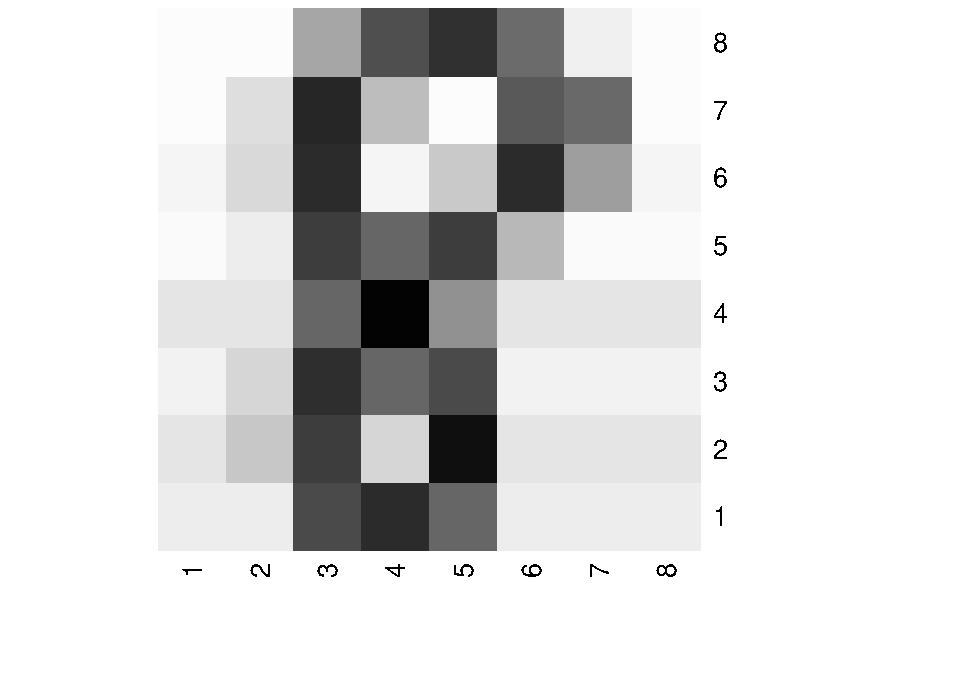
\includegraphics{lab1_report_files/figure-latex/1.3.3-1.pdf}
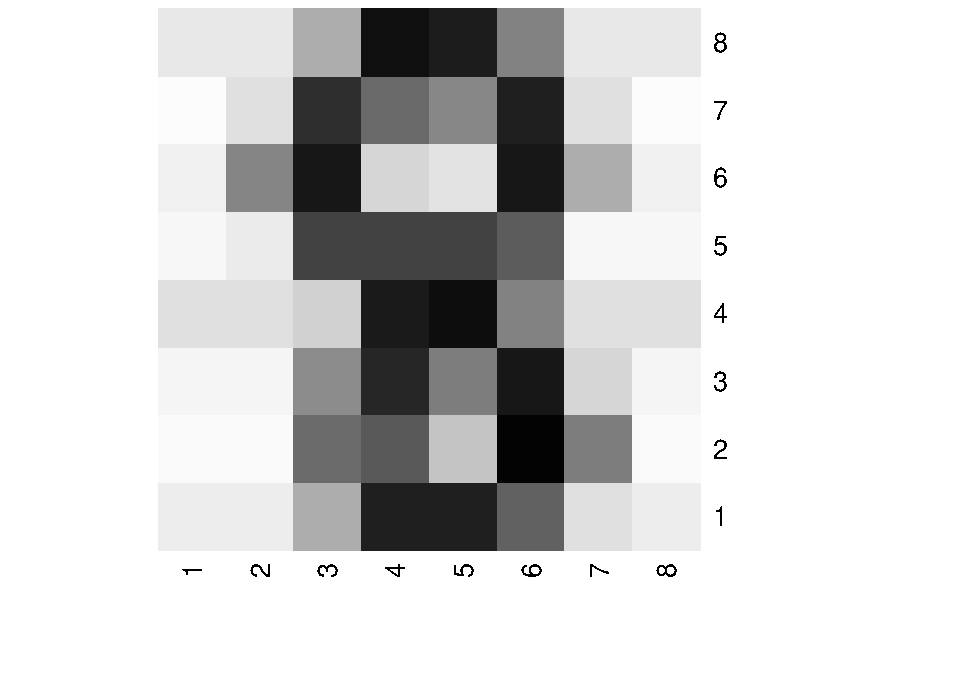
\includegraphics{lab1_report_files/figure-latex/1.3.3-2.pdf}

\begin{Shaded}
\begin{Highlighting}[]
\CommentTok{\#Low probabilities}
\ControlFlowTok{for}\NormalTok{(i }\ControlFlowTok{in} \DecValTok{1}\SpecialCharTok{:}\DecValTok{3}\NormalTok{)\{}
  \FunctionTok{visualise\_dig}\NormalTok{(low\_idx[i], digits\_train)}
\NormalTok{\}}
\end{Highlighting}
\end{Shaded}

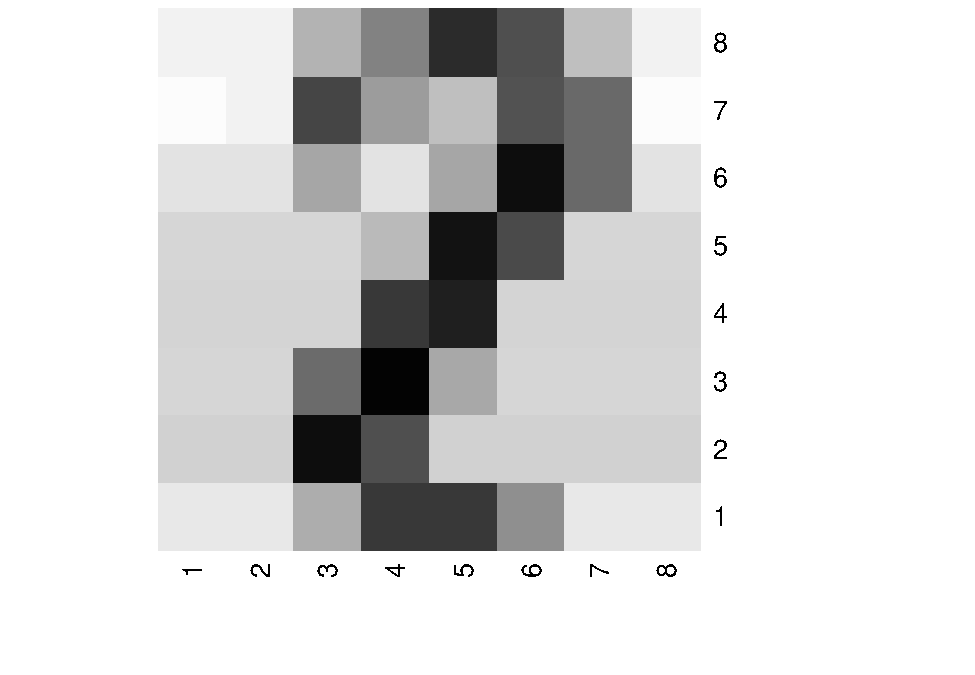
\includegraphics{lab1_report_files/figure-latex/1.3.3-3.pdf}
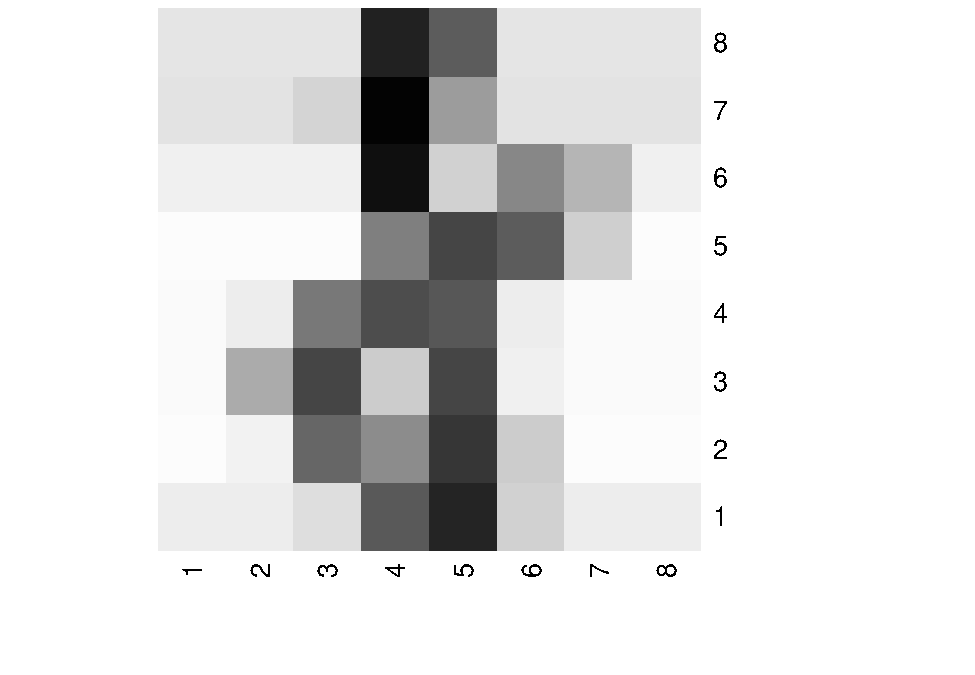
\includegraphics{lab1_report_files/figure-latex/1.3.3-4.pdf}
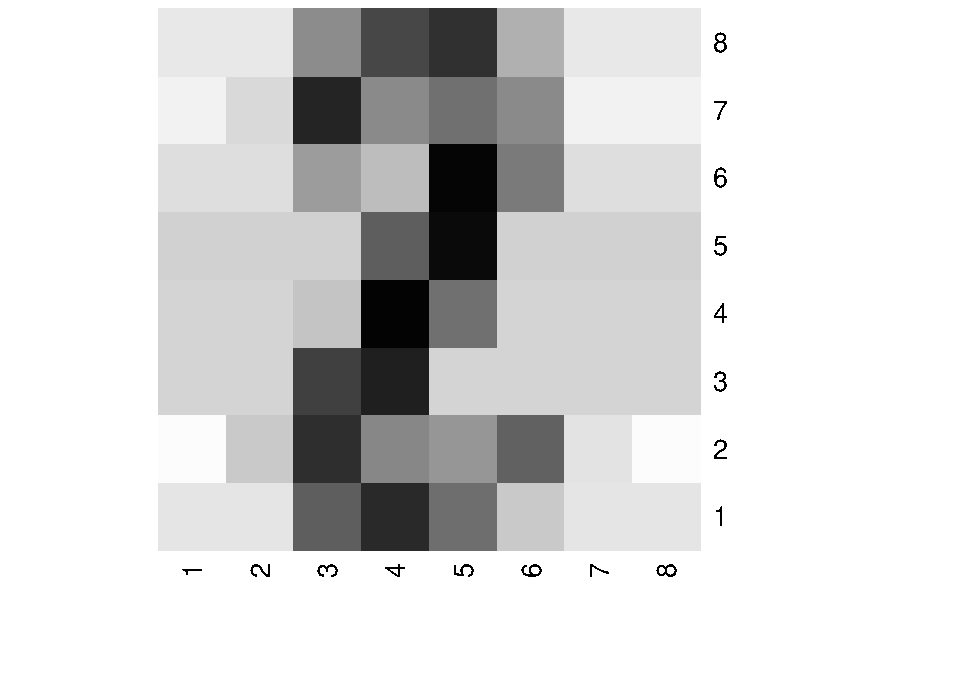
\includegraphics{lab1_report_files/figure-latex/1.3.3-5.pdf}

\hypertarget{section-3}{%
\subsection{4.}\label{section-3}}

\begin{quote}
Fit a K-nearest neighbor classifiers to the training data for different
values of K K = 1,2, \ldots{} , 30 and plot the dependence of the
training and validation misclassification errors on the value of K (in
the same plot). How does the model complexity change when K increases
and how does it affect the training and validation errors? Report the
optimal K K according to this plot. Finally, estimate the test error for
the model having the optimal K, compare it with the training and
validation errors and make necessary conclusions about the model
quality.
\end{quote}

\begin{Shaded}
\begin{Highlighting}[]
\NormalTok{k\_values }\OtherTok{\textless{}{-}} \FunctionTok{c}\NormalTok{()}
\NormalTok{misc\_errs\_test }\OtherTok{\textless{}{-}} \FunctionTok{c}\NormalTok{()}
\NormalTok{misc\_errs\_train }\OtherTok{\textless{}{-}} \FunctionTok{c}\NormalTok{()}

\ControlFlowTok{for}\NormalTok{(i }\ControlFlowTok{in} \FunctionTok{c}\NormalTok{(}\DecValTok{1}\SpecialCharTok{:}\DecValTok{30}\NormalTok{))\{}
  \CommentTok{\#Fitting the classifier}
  \CommentTok{\#Test:}
\NormalTok{  digits\_kknn\_test\_i }\OtherTok{\textless{}{-}} \FunctionTok{kknn}\NormalTok{(}\AttributeTok{formula =} \FunctionTok{as.factor}\NormalTok{(V65) }\SpecialCharTok{\textasciitilde{}}\NormalTok{ . , }\AttributeTok{train =}\NormalTok{ digits\_train, }\AttributeTok{test =}\NormalTok{ digits\_valid, }\AttributeTok{k =}\NormalTok{ i, }\AttributeTok{kernel =} \StringTok{"rectangular"}\NormalTok{)}
  \CommentTok{\#Train:}
\NormalTok{  digits\_kknn\_train\_i }\OtherTok{\textless{}{-}} \FunctionTok{kknn}\NormalTok{(}\AttributeTok{formula =} \FunctionTok{as.factor}\NormalTok{(V65) }\SpecialCharTok{\textasciitilde{}}\NormalTok{ . , }\AttributeTok{train =}\NormalTok{ digits\_train, }\AttributeTok{test =}\NormalTok{ digits\_train, }\AttributeTok{k =}\NormalTok{ i, }\AttributeTok{kernel =} \StringTok{"rectangular"}\NormalTok{)}
  
  \CommentTok{\#kbetter \textless{}{-} train.kknn(formula = as.factor(V65) \textasciitilde{} . , data = digits\_train, ks=i, kernel = "rectangular")}
  \CommentTok{\#Predicting the values}
\NormalTok{  fitted\_values\_valid }\OtherTok{\textless{}{-}} \FunctionTok{predict}\NormalTok{(digits\_kknn\_test\_i, }\AttributeTok{data =}\NormalTok{ digits\_valid)}
\NormalTok{  fitted\_values\_train }\OtherTok{\textless{}{-}} \FunctionTok{predict}\NormalTok{(digits\_kknn\_train\_i, }\AttributeTok{data =}\NormalTok{ digits\_train)}
  \CommentTok{\#Confusion matrix}
\NormalTok{  conf\_mat\_test }\OtherTok{\textless{}{-}} \FunctionTok{table}\NormalTok{(}\AttributeTok{obs =}\NormalTok{ digits\_valid}\SpecialCharTok{$}\NormalTok{V65, }\AttributeTok{pred =}\NormalTok{ fitted\_values\_valid)}
\NormalTok{  conf\_mat\_train }\OtherTok{\textless{}{-}} \FunctionTok{table}\NormalTok{(}\AttributeTok{obs =}\NormalTok{ digits\_train}\SpecialCharTok{$}\NormalTok{V65, }\AttributeTok{pred =}\NormalTok{ fitted\_values\_train)}
  \CommentTok{\#Misclassification error}
\NormalTok{  misc\_err\_test }\OtherTok{\textless{}{-}} \FunctionTok{get\_mean\_misc\_err}\NormalTok{(conf\_mat\_test)}
\NormalTok{  misc\_err\_train }\OtherTok{\textless{}{-}} \FunctionTok{get\_mean\_misc\_err}\NormalTok{(conf\_mat\_train)}
  
  \CommentTok{\#Append to the vectors}
\NormalTok{  k\_values }\OtherTok{\textless{}{-}} \FunctionTok{append}\NormalTok{(k\_values, i)}
\NormalTok{  misc\_errs\_test }\OtherTok{\textless{}{-}} \FunctionTok{append}\NormalTok{(misc\_errs\_test, misc\_err\_test)}
\NormalTok{  misc\_errs\_train }\OtherTok{\textless{}{-}} \FunctionTok{append}\NormalTok{(misc\_errs\_train, misc\_err\_train)}
\NormalTok{\}}
\NormalTok{df\_ks }\OtherTok{\textless{}{-}} \FunctionTok{data.frame}\NormalTok{(}\StringTok{"k"} \OtherTok{=}\NormalTok{ k\_values, }\StringTok{"misc\_err\_test"} \OtherTok{=}\NormalTok{ misc\_errs\_test, }\StringTok{"misc\_err\_train"} \OtherTok{=}\NormalTok{ misc\_errs\_train)}
\end{Highlighting}
\end{Shaded}

\begin{Shaded}
\begin{Highlighting}[]
\FunctionTok{library}\NormalTok{(ggplot2)}
\CommentTok{\#Plotting misc\_errs\_test and misc\_errs\_train as a function of k}
\FunctionTok{ggplot}\NormalTok{(df\_ks, }\FunctionTok{aes}\NormalTok{(}\AttributeTok{x =}\NormalTok{ k, }\AttributeTok{y =}\NormalTok{ misc\_err\_test)) }\SpecialCharTok{+} \FunctionTok{geom\_line}\NormalTok{() }\SpecialCharTok{+} \FunctionTok{geom\_point}\NormalTok{() }\SpecialCharTok{+} \FunctionTok{geom\_line}\NormalTok{(}\FunctionTok{aes}\NormalTok{(}\AttributeTok{y =}\NormalTok{ misc\_err\_train), }\AttributeTok{color =} \StringTok{"red"}\NormalTok{) }\SpecialCharTok{+} \FunctionTok{geom\_point}\NormalTok{(}\FunctionTok{aes}\NormalTok{(}\AttributeTok{y =}\NormalTok{ misc\_err\_train), }\AttributeTok{color =} \StringTok{"red"}\NormalTok{) }\SpecialCharTok{+} \FunctionTok{ggtitle}\NormalTok{(}\StringTok{"Misc error as a function of k"}\NormalTok{) }\SpecialCharTok{+} \FunctionTok{xlab}\NormalTok{(}\StringTok{"k"}\NormalTok{) }\SpecialCharTok{+} \FunctionTok{ylab}\NormalTok{(}\StringTok{"Misc error"}\NormalTok{)}
\end{Highlighting}
\end{Shaded}

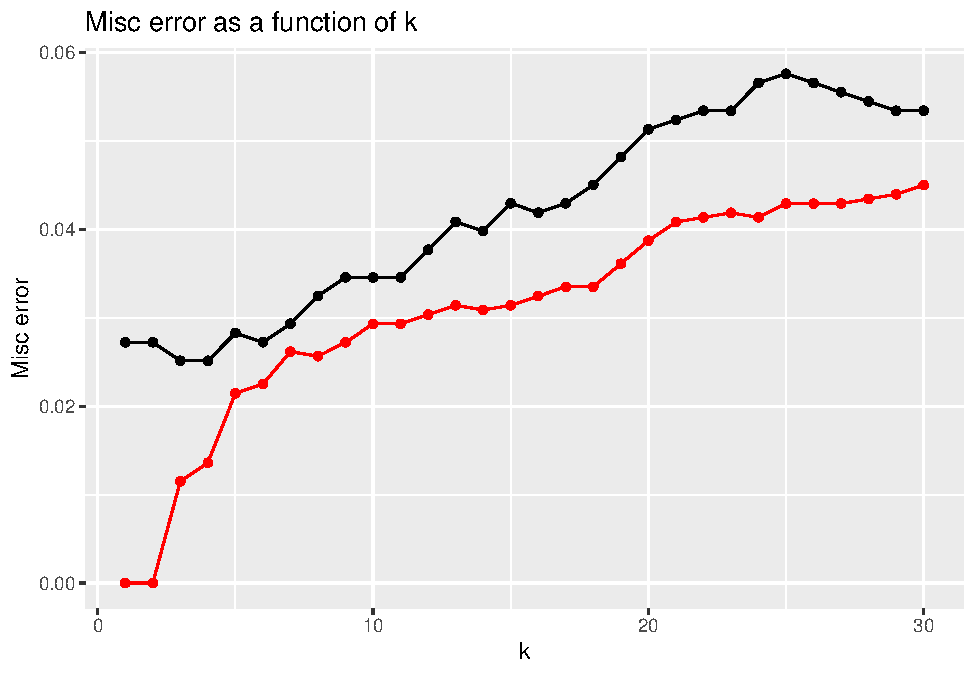
\includegraphics{lab1_report_files/figure-latex/1.4 plot-1.pdf}

It would seems like k=3 and k=4 have the lowest valid misclassification
rate. Since k=3 have a lower training misclassification rate, we choose
k=3 as the optimal k. The model complexity increases with k but it does
not seem to affect the training and validation errors after k=3.

\begin{Shaded}
\begin{Highlighting}[]
\CommentTok{\#Estimation of the model for k=3}

\CommentTok{\#Fitting the classifier}
\NormalTok{digits\_kknn\_test\_3 }\OtherTok{\textless{}{-}} \FunctionTok{kknn}\NormalTok{(}\AttributeTok{formula =} \FunctionTok{as.factor}\NormalTok{(V65) }\SpecialCharTok{\textasciitilde{}}\NormalTok{ . , }\AttributeTok{train =}\NormalTok{ digits\_train, }\AttributeTok{test =}\NormalTok{ digits\_test, }\AttributeTok{k =} \DecValTok{3}\NormalTok{, }\AttributeTok{kernel =} \StringTok{"rectangular"}\NormalTok{)}
\NormalTok{digits\_kknn\_train\_3 }\OtherTok{\textless{}{-}} \FunctionTok{kknn}\NormalTok{(}\AttributeTok{formula =} \FunctionTok{as.factor}\NormalTok{(V65) }\SpecialCharTok{\textasciitilde{}}\NormalTok{ . , }\AttributeTok{train =}\NormalTok{ digits\_train, }\AttributeTok{test =}\NormalTok{ digits\_train, }\AttributeTok{k =} \DecValTok{3}\NormalTok{, }\AttributeTok{kernel =} \StringTok{"rectangular"}\NormalTok{)}
\NormalTok{digits\_kknn\_valid\_3 }\OtherTok{\textless{}{-}} \FunctionTok{kknn}\NormalTok{(}\AttributeTok{formula =} \FunctionTok{as.factor}\NormalTok{(V65) }\SpecialCharTok{\textasciitilde{}}\NormalTok{ . , }\AttributeTok{train =}\NormalTok{ digits\_train, }\AttributeTok{test =}\NormalTok{ digits\_valid, }\AttributeTok{k =} \DecValTok{3}\NormalTok{, }\AttributeTok{kernel =} \StringTok{"rectangular"}\NormalTok{)}

\CommentTok{\#Predicting the values}
\NormalTok{fitted\_values\_test\_3 }\OtherTok{\textless{}{-}} \FunctionTok{predict}\NormalTok{(digits\_kknn\_test\_3, }\AttributeTok{data =}\NormalTok{ digits\_test)}
\NormalTok{fitted\_values\_train\_3 }\OtherTok{\textless{}{-}} \FunctionTok{predict}\NormalTok{(digits\_kknn\_train\_3, }\AttributeTok{data =}\NormalTok{ digits\_train)}
\NormalTok{fitted\_values\_valid\_3 }\OtherTok{\textless{}{-}} \FunctionTok{predict}\NormalTok{(digits\_kknn\_valid\_3, }\AttributeTok{data =}\NormalTok{ digits\_valid)}
\CommentTok{\#Validation error}
\NormalTok{conf\_mat\_test\_3 }\OtherTok{\textless{}{-}} \FunctionTok{table}\NormalTok{(}\AttributeTok{obs =}\NormalTok{ digits\_test}\SpecialCharTok{$}\NormalTok{V65, }\AttributeTok{pred =}\NormalTok{ fitted\_values\_test\_3)}
\NormalTok{conf\_mat\_train\_3 }\OtherTok{\textless{}{-}} \FunctionTok{table}\NormalTok{(}\AttributeTok{obs =}\NormalTok{ digits\_train}\SpecialCharTok{$}\NormalTok{V65, }\AttributeTok{pred =}\NormalTok{ fitted\_values\_train\_3)}
\NormalTok{conf\_mat\_valid\_3 }\OtherTok{\textless{}{-}} \FunctionTok{table}\NormalTok{(}\AttributeTok{obs =}\NormalTok{ digits\_valid}\SpecialCharTok{$}\NormalTok{V65, }\AttributeTok{pred =}\NormalTok{ fitted\_values\_valid\_3)}
\CommentTok{\#Misclassification error}
\NormalTok{misc\_err\_test\_3 }\OtherTok{\textless{}{-}} \FunctionTok{get\_mean\_misc\_err}\NormalTok{(conf\_mat\_test\_3)}
\NormalTok{misc\_err\_train\_3 }\OtherTok{\textless{}{-}} \FunctionTok{get\_mean\_misc\_err}\NormalTok{(conf\_mat\_train\_3)}
\NormalTok{misc\_err\_valid\_3 }\OtherTok{\textless{}{-}} \FunctionTok{get\_mean\_misc\_err}\NormalTok{(conf\_mat\_valid\_3)}

\FunctionTok{print}\NormalTok{(}\FunctionTok{paste}\NormalTok{(}\StringTok{"Test error for k=3: "}\NormalTok{, misc\_err\_test\_3))}
\end{Highlighting}
\end{Shaded}

\begin{verbatim}
## [1] "Test error for k=3:  0.0240334378265413"
\end{verbatim}

\begin{Shaded}
\begin{Highlighting}[]
\FunctionTok{print}\NormalTok{(}\FunctionTok{paste}\NormalTok{(}\StringTok{"Train error for k=3: "}\NormalTok{, misc\_err\_train\_3))}
\end{Highlighting}
\end{Shaded}

\begin{verbatim}
## [1] "Train error for k=3:  0.0115122972265829"
\end{verbatim}

\begin{Shaded}
\begin{Highlighting}[]
\FunctionTok{print}\NormalTok{(}\FunctionTok{paste}\NormalTok{(}\StringTok{"Valid error for k=3: "}\NormalTok{, misc\_err\_valid\_3))}
\end{Highlighting}
\end{Shaded}

\begin{verbatim}
## [1] "Valid error for k=3:  0.025130890052356"
\end{verbatim}

\hypertarget{section-4}{%
\subsection{5.}\label{section-4}}

\begin{quote}
Fit K-nearest neighbor classifiers to the training data for different
values of K K = 1,2, \ldots{} , 30, compute the error for the validation
data as cross-entropy (when computing log of probabilities add a small
constant within log, e.g.~1e-15, to avoid numerical problems) and plot
the dependence of the validation error on the value of K K.
\end{quote}

Cross Entropy :
\[J(y,\hat{p}(y)) = -\sum_{i=1}^{n}\sum_{m=1}^{M}I(y_i=C_m)*log(\hat{p}(y_i=C_m))\]

\begin{Shaded}
\begin{Highlighting}[]
\NormalTok{get\_cross\_entropy }\OtherTok{\textless{}{-}} \ControlFlowTok{function}\NormalTok{(prob, true\_vals)\{}
\NormalTok{  ce\_sum }\OtherTok{\textless{}{-}} \DecValTok{0}
  \ControlFlowTok{for}\NormalTok{(i }\ControlFlowTok{in} \DecValTok{1}\SpecialCharTok{:}\FunctionTok{length}\NormalTok{(true\_vals))\{ }\CommentTok{\#for each prediction}
\NormalTok{    truth }\OtherTok{\textless{}{-}}\NormalTok{ true\_vals[i] }\CommentTok{\#Cm}
\NormalTok{    ce\_sum }\OtherTok{\textless{}{-}}\NormalTok{ ce\_sum }\SpecialCharTok{+} \FunctionTok{log}\NormalTok{(prob[i,truth}\SpecialCharTok{+}\DecValTok{1}\NormalTok{] }\SpecialCharTok{+} \FloatTok{1e{-}15}\NormalTok{)}
\NormalTok{  \}}
  \FunctionTok{return}\NormalTok{ (}\SpecialCharTok{{-}}\DecValTok{1}\SpecialCharTok{*}\NormalTok{ce\_sum)}
\NormalTok{\}}
\NormalTok{k\_values }\OtherTok{\textless{}{-}} \FunctionTok{c}\NormalTok{()}
\NormalTok{x\_ent\_errs }\OtherTok{\textless{}{-}} \FunctionTok{c}\NormalTok{()}
\ControlFlowTok{for}\NormalTok{(i }\ControlFlowTok{in} \DecValTok{1}\SpecialCharTok{:}\DecValTok{30}\NormalTok{)\{}
  \CommentTok{\#Fitting the classifier}
  \FunctionTok{cat}\NormalTok{(i, }\StringTok{" "}\NormalTok{)}
  \CommentTok{\#Valid:}
\NormalTok{  digits\_kknn\_ce }\OtherTok{\textless{}{-}} \FunctionTok{kknn}\NormalTok{(}\AttributeTok{formula =} \FunctionTok{as.factor}\NormalTok{(V65) }\SpecialCharTok{\textasciitilde{}}\NormalTok{ . , }\AttributeTok{train =}\NormalTok{ digits\_train, }\AttributeTok{test =}\NormalTok{ digits\_valid, }\AttributeTok{k =}\NormalTok{ i, }\AttributeTok{kernel =} \StringTok{"rectangular"}\NormalTok{)}

  \CommentTok{\#Cross entropy Error:}
\NormalTok{  ce\_err }\OtherTok{\textless{}{-}} \FunctionTok{get\_cross\_entropy}\NormalTok{(digits\_kknn\_ce[[}\StringTok{"prob"}\NormalTok{]], digits\_valid}\SpecialCharTok{$}\NormalTok{V65)}
  \CommentTok{\#Append to the vectors}
\NormalTok{  k\_values }\OtherTok{\textless{}{-}} \FunctionTok{append}\NormalTok{(k\_values, i)}
\NormalTok{  x\_ent\_errs }\OtherTok{\textless{}{-}} \FunctionTok{append}\NormalTok{(x\_ent\_errs, ce\_err)}
\NormalTok{\}}
\end{Highlighting}
\end{Shaded}

\begin{verbatim}
## 1  2  3  4  5  6  7  8  9  10  11  12  13  14  15  16  17  18  19  20  21  22  23  24  25  26  27  28  29  30
\end{verbatim}

\begin{Shaded}
\begin{Highlighting}[]
\NormalTok{df\_CE }\OtherTok{\textless{}{-}} \FunctionTok{data.frame}\NormalTok{(}\StringTok{"k"} \OtherTok{=}\NormalTok{ k\_values, }\StringTok{"CE\_err"} \OtherTok{=}\NormalTok{ x\_ent\_errs)}
\end{Highlighting}
\end{Shaded}

Plot:

\begin{Shaded}
\begin{Highlighting}[]
\CommentTok{\#Plotting misc\_errs\_test and misc\_errs\_train as a function of k}
\FunctionTok{ggplot}\NormalTok{(df\_CE, }\FunctionTok{aes}\NormalTok{(}\AttributeTok{x =}\NormalTok{ k, }\AttributeTok{y =}\NormalTok{ CE\_err)) }\SpecialCharTok{+} \FunctionTok{geom\_line}\NormalTok{() }\SpecialCharTok{+} \FunctionTok{geom\_point}\NormalTok{() }\SpecialCharTok{+} \FunctionTok{ggtitle}\NormalTok{(}\StringTok{"Cross Entropy error as a function of k"}\NormalTok{) }\SpecialCharTok{+} \FunctionTok{xlab}\NormalTok{(}\StringTok{"k"}\NormalTok{) }\SpecialCharTok{+} \FunctionTok{ylab}\NormalTok{(}\StringTok{"CE error"}\NormalTok{)}
\end{Highlighting}
\end{Shaded}

\includegraphics{lab1_report_files/figure-latex/unnamed-chunk-2-1.pdf}

\begin{quote}
What is the optimal K K value here? Assuming that response has
multinomial distribution, why might the cross-entropy be a more suitable
choice of the error function than the misclassification error for this
problem?
\end{quote}

\begin{center}\rule{0.5\linewidth}{0.5pt}\end{center}

\hypertarget{assignment-2}{%
\section{Assignment 2}\label{assignment-2}}

\hypertarget{section-5}{%
\subsection{2.1}\label{section-5}}

\begin{quote}
Divide it into training and test data (60/40) and scale it
appropriately. In the coming steps, assume that motor\_UPDRS is normally
distributed and is a function of the voice characteristics, and since
the data are scaled, no intercept is needed in the modelling.
\end{quote}

\begin{Shaded}
\begin{Highlighting}[]
\CommentTok{\# Read in data}
\NormalTok{df\_park }\OtherTok{\textless{}{-}} \FunctionTok{read.csv}\NormalTok{(}\StringTok{"parkinsons.csv"}\NormalTok{)}

\CommentTok{\# Split training/test and scale}
\FunctionTok{set.seed}\NormalTok{(}\DecValTok{12345}\NormalTok{)}
\NormalTok{train\_ind }\OtherTok{\textless{}{-}} \FunctionTok{sample}\NormalTok{(}\DecValTok{1}\SpecialCharTok{:}\FunctionTok{nrow}\NormalTok{(df\_park), }\FunctionTok{floor}\NormalTok{(}\FunctionTok{nrow}\NormalTok{(df\_park) }\SpecialCharTok{*} \FloatTok{0.6}\NormalTok{))}
\NormalTok{df\_train }\OtherTok{\textless{}{-}}\NormalTok{ df\_park[train\_ind,]}
\NormalTok{df\_test }\OtherTok{\textless{}{-}}\NormalTok{ df\_park[}\SpecialCharTok{{-}}\NormalTok{train\_ind,]}

\NormalTok{scaler }\OtherTok{\textless{}{-}} \FunctionTok{preProcess}\NormalTok{(df\_train)}
\NormalTok{df\_train\_scaled }\OtherTok{\textless{}{-}} \FunctionTok{predict}\NormalTok{(scaler, df\_train)}
\NormalTok{df\_test\_scaled }\OtherTok{\textless{}{-}} \FunctionTok{predict}\NormalTok{(scaler, df\_test)}
\end{Highlighting}
\end{Shaded}

\hypertarget{section-6}{%
\subsection{2.2}\label{section-6}}

\begin{quote}
Compute a linear regression model from the training data, estimate
training and test MSE and comment on which variables contribute
significantly to the model.
\end{quote}

\begin{verbatim}
## MSE training data: 0.8785431
## MSE test data: 0.9354477
\end{verbatim}

\begin{verbatim}
## 
## Call:
## lm(formula = motor_UPDRS ~ . + 0 - subject. - age - sex - test_time - 
##     total_UPDRS, data = df_train_scaled)
## 
## Residuals:
##     Min      1Q  Median      3Q     Max 
## -3.0255 -0.7363 -0.1087  0.7333  2.1960 
## 
## Coefficients:
##                 Estimate Std. Error t value Pr(>|t|)    
## Jitter...       0.186931   0.149561   1.250 0.211431    
## Jitter.Abs.    -0.169609   0.040805  -4.157 3.31e-05 ***
## Jitter.RAP     -5.269544  18.834160  -0.280 0.779658    
## Jitter.PPQ5    -0.074568   0.087766  -0.850 0.395592    
## Jitter.DDP      5.249558  18.837525   0.279 0.780510    
## Shimmer         0.592436   0.205981   2.876 0.004050 ** 
## Shimmer.dB.    -0.172655   0.139316  -1.239 0.215315    
## Shimmer.APQ3   32.070932  77.159242   0.416 0.677694    
## Shimmer.APQ5   -0.387507   0.113789  -3.405 0.000668 ***
## Shimmer.APQ11   0.305546   0.061236   4.990 6.34e-07 ***
## Shimmer.DDA   -32.387241  77.158814  -0.420 0.674695    
## NHR            -0.185387   0.045567  -4.068 4.84e-05 ***
## HNR            -0.238543   0.036395  -6.554 6.41e-11 ***
## RPDE            0.004068   0.022664   0.179 0.857556    
## DFA            -0.280318   0.020136 -13.921  < 2e-16 ***
## PPE             0.226467   0.032881   6.887 6.70e-12 ***
## ---
## Signif. codes:  0 '***' 0.001 '**' 0.01 '*' 0.05 '.' 0.1 ' ' 1
## 
## Residual standard error: 0.9394 on 3509 degrees of freedom
## Multiple R-squared:  0.1212, Adjusted R-squared:  0.1172 
## F-statistic: 30.25 on 16 and 3509 DF,  p-value: < 2.2e-16
\end{verbatim}

The total\_UPDRS variables has by far the biggest impact on the model.
If this variable is included in the model, the MSE on both the training
and test data are very good at about 0.09. The MSE on the test data is
slightly higher than it is on the training data, which suggests the
model was not overfit to the training data. However, when this variable
is removed from the model, the MSE rises from 0.09 to about 0.8-0.9.
There is no description of the variable included in the assignment, but
it may be very strongly, if not fully correlated with motor\_UPDRS,
causing it to be the main predictor in the model. If this is the case,
it is probably a bad idea to include this variable in the model, as it
pretty much represents the same thing as the y variable.

Either way, though, there are quite a few variables that are not
significant. When including total\_UPDRS in the model, Jitter.Abs.,
Jitter.DDP, Shimmer.APQ3, Shimmer.DDA, NHR, and HNR all have p-values
above 0.7, and test\_time, Jitter.PPQ5, Shimmer.dB., and DFA are also
not significant. Not much pre-exploring of the data was done in the
assignment before putting together the model, but it would be good to
check if there is any multicollinearity happening within the Jitter and
Shimmer categories. Similarly, NHR and HNR are similar measures and may
be capturing the same information. When total\_UPDRS is removed,
Jiter.RAP, Jitter.DDP, and RPDE have very high p-values, and
Jitter\ldots, Jitter.PPQ5, Shimmer.dB., Shimmer.APQ3, and Shimmer.DDA
are also not significant. While not being significant, Shimmer.APQ3 has
the largest coefficient value, meaning it has the biggest impact on the
prediction.

\hypertarget{a}{%
\subsection{2.3a}\label{a}}

\begin{quote}
Loglikelihood function that for a given parameter vector 𝜽 and
dispersion 𝜎 computes the log-likelihood function log 𝑃(𝑇\textbar 𝜽, 𝜎)
for the stated model and the training data.
\end{quote}

\begin{Shaded}
\begin{Highlighting}[]
\NormalTok{loglikelihood }\OtherTok{\textless{}{-}} \ControlFlowTok{function}\NormalTok{(data, formula, theta, sigma) \{}
  \CommentTok{\# Get variable names and y and x matrices}
\NormalTok{  y\_var }\OtherTok{\textless{}{-}} \FunctionTok{all.vars}\NormalTok{(formula)[}\DecValTok{1}\NormalTok{]}
\NormalTok{  x\_var }\OtherTok{\textless{}{-}} \FunctionTok{all.vars}\NormalTok{(formula)[}\DecValTok{2}\SpecialCharTok{:}\FunctionTok{length}\NormalTok{(}\FunctionTok{all.vars}\NormalTok{(formula))]}
  
  \ControlFlowTok{if}\NormalTok{ (}\StringTok{"."} \SpecialCharTok{\%in\%}\NormalTok{ x\_var) \{}
\NormalTok{    x\_var\_sub }\OtherTok{\textless{}{-}}\NormalTok{ x\_var[x\_var }\SpecialCharTok{!=} \StringTok{"."}\NormalTok{]}
\NormalTok{    x\_var }\OtherTok{\textless{}{-}} \FunctionTok{colnames}\NormalTok{(data)[}\FunctionTok{colnames}\NormalTok{(data) }\SpecialCharTok{!=}\NormalTok{ y\_var]}
\NormalTok{    x\_var }\OtherTok{\textless{}{-}}\NormalTok{ x\_var[}\SpecialCharTok{!}\NormalTok{(x\_var }\SpecialCharTok{\%in\%}\NormalTok{ x\_var\_sub)]}
\NormalTok{  \}}
  
\NormalTok{  y }\OtherTok{\textless{}{-}}\NormalTok{ data[, y\_var]}
\NormalTok{  x }\OtherTok{\textless{}{-}}\NormalTok{ data[, x\_var]}
  
  \CommentTok{\# Get n observations}
\NormalTok{  n }\OtherTok{\textless{}{-}} \FunctionTok{nrow}\NormalTok{(data)}
  
  \CommentTok{\# Compute log likelihood}
\NormalTok{  log\_likelihood }\OtherTok{\textless{}{-}} \SpecialCharTok{{-}}\NormalTok{n }\SpecialCharTok{*} \FunctionTok{log}\NormalTok{(}\FunctionTok{sqrt}\NormalTok{(}\DecValTok{2} \SpecialCharTok{*}\NormalTok{ pi }\SpecialCharTok{*}\NormalTok{ sigma}\SpecialCharTok{\^{}}\DecValTok{2}\NormalTok{)) }\SpecialCharTok{{-}} \DecValTok{1} \SpecialCharTok{/}\NormalTok{ (}\DecValTok{2} \SpecialCharTok{*}\NormalTok{ sigma}\SpecialCharTok{\^{}}\DecValTok{2}\NormalTok{) }\SpecialCharTok{*} \FunctionTok{sum}\NormalTok{((y }\SpecialCharTok{{-}} \FunctionTok{t}\NormalTok{(theta) }\SpecialCharTok{*}\NormalTok{ x)}\SpecialCharTok{\^{}}\DecValTok{2}\NormalTok{)}
  
  \FunctionTok{return}\NormalTok{(log\_likelihood)}
\NormalTok{\}}
\end{Highlighting}
\end{Shaded}

\hypertarget{b}{%
\subsection{2.3b}\label{b}}

\begin{quote}
Ridge function that for given vector 𝜽, scalar 𝜎 and scalar 𝜆 uses
function from 3a and adds up a Ridge penalty 𝜆‖𝜽‖\^{}2 to the minus
log-likelihood.
\end{quote}

\begin{Shaded}
\begin{Highlighting}[]
\NormalTok{ridge }\OtherTok{\textless{}{-}} \ControlFlowTok{function}\NormalTok{(v\_theta\_sigma, data, formula, lambda) \{}
\NormalTok{  theta }\OtherTok{\textless{}{-}}\NormalTok{ v\_theta\_sigma[}\DecValTok{1}\SpecialCharTok{:}\FunctionTok{length}\NormalTok{(v\_theta\_sigma) }\SpecialCharTok{{-}} \DecValTok{1}\NormalTok{]}
\NormalTok{  sigma }\OtherTok{\textless{}{-}}\NormalTok{ v\_theta\_sigma[}\FunctionTok{length}\NormalTok{(v\_theta\_sigma)]}
  
\NormalTok{  penalty }\OtherTok{\textless{}{-}}\NormalTok{ lambda }\SpecialCharTok{*} \FunctionTok{sum}\NormalTok{(theta}\SpecialCharTok{\^{}}\DecValTok{2}\NormalTok{) }\CommentTok{\# https://stackoverflow.com/questions/10933945/how{-}to{-}calculate{-}the{-}euclidean{-}norm{-}of{-}a{-}vector{-}in{-}r}
\NormalTok{  min\_loglikelihood }\OtherTok{\textless{}{-}} \SpecialCharTok{{-}}\FunctionTok{loglikelihood}\NormalTok{(data, formula, theta, sigma)}
\NormalTok{  penalized\_min\_loglikelihood }\OtherTok{\textless{}{-}}\NormalTok{ min\_loglikelihood }\SpecialCharTok{+}\NormalTok{ penalty}
  
  \FunctionTok{return}\NormalTok{(penalized\_min\_loglikelihood)}
\NormalTok{\}}
\end{Highlighting}
\end{Shaded}

\hypertarget{c}{%
\subsection{2.3c}\label{c}}

\begin{quote}
RidgeOptfunction that depends on scalar 𝜆, uses function from 3b and
function optim() with method=''BFGS'' to find the optimal 𝜽 and 𝜎 for
the given 𝜆.
\end{quote}

\begin{Shaded}
\begin{Highlighting}[]
\NormalTok{ridge\_opt }\OtherTok{\textless{}{-}} \ControlFlowTok{function}\NormalTok{(data, formula, lambda) \{}
  \CommentTok{\# \# https://stackoverflow.com/questions/24623488/how{-}do{-}i{-}use{-}a{-}function{-}with{-}parameters{-}in{-}optim{-}in{-}r}
  \CommentTok{\# https://stackoverflow.com/questions/59517244/r{-}optim{-}can{-}i{-}pass{-}a{-}list{-}to{-}parameter{-}par}
\NormalTok{  y\_var }\OtherTok{\textless{}{-}} \FunctionTok{all.vars}\NormalTok{(formula)[}\DecValTok{1}\NormalTok{]}
\NormalTok{  x\_var }\OtherTok{\textless{}{-}} \FunctionTok{all.vars}\NormalTok{(formula)[}\DecValTok{2}\SpecialCharTok{:}\FunctionTok{length}\NormalTok{(}\FunctionTok{all.vars}\NormalTok{(formula))]}
  
  \ControlFlowTok{if}\NormalTok{ (}\StringTok{"."} \SpecialCharTok{\%in\%}\NormalTok{ x\_var) \{}
\NormalTok{    x\_var\_sub }\OtherTok{\textless{}{-}}\NormalTok{ x\_var[x\_var }\SpecialCharTok{!=} \StringTok{"."}\NormalTok{]}
\NormalTok{    x\_var }\OtherTok{\textless{}{-}} \FunctionTok{colnames}\NormalTok{(data)[}\FunctionTok{colnames}\NormalTok{(data) }\SpecialCharTok{!=}\NormalTok{ y\_var]}
\NormalTok{    x\_var }\OtherTok{\textless{}{-}}\NormalTok{ x\_var[}\SpecialCharTok{!}\NormalTok{(x\_var }\SpecialCharTok{\%in\%}\NormalTok{ x\_var\_sub)]}
\NormalTok{  \}}
  
\NormalTok{  opt }\OtherTok{\textless{}{-}} \FunctionTok{optim}\NormalTok{(}\FunctionTok{c}\NormalTok{(}\FunctionTok{rep}\NormalTok{(}\DecValTok{0}\NormalTok{, }\FunctionTok{length}\NormalTok{(x\_var)), }\DecValTok{1}\NormalTok{), ridge, }\AttributeTok{data=}\NormalTok{data, }\AttributeTok{formula=}\NormalTok{formula, }\AttributeTok{lambda=}\NormalTok{lambda, }\AttributeTok{method=}\StringTok{"BFGS"}\NormalTok{)}
\NormalTok{  opt\_theta }\OtherTok{\textless{}{-}}\NormalTok{ opt}\SpecialCharTok{$}\NormalTok{par[}\DecValTok{1}\SpecialCharTok{:}\FunctionTok{length}\NormalTok{(opt}\SpecialCharTok{$}\NormalTok{par) }\SpecialCharTok{{-}} \DecValTok{1}\NormalTok{]}
\NormalTok{  opt\_sigma }\OtherTok{\textless{}{-}}\NormalTok{ opt}\SpecialCharTok{$}\NormalTok{par[}\FunctionTok{length}\NormalTok{(opt}\SpecialCharTok{$}\NormalTok{par)]}
  
  \FunctionTok{return}\NormalTok{(}\FunctionTok{list}\NormalTok{(}\AttributeTok{theta=}\NormalTok{opt\_theta, }\AttributeTok{sigma=}\NormalTok{opt\_sigma))}
\NormalTok{\}}
\end{Highlighting}
\end{Shaded}

\hypertarget{d}{%
\subsection{2.3d}\label{d}}

\begin{quote}
Df function that for a given scalar 𝜆 computes the degrees of freedom of
the Ridge model based on the training data.
\end{quote}

\begin{Shaded}
\begin{Highlighting}[]
\NormalTok{df }\OtherTok{\textless{}{-}} \ControlFlowTok{function}\NormalTok{(data, formula, lambda) \{}
  \CommentTok{\# Get x matrix}
\NormalTok{  y\_var }\OtherTok{\textless{}{-}} \FunctionTok{all.vars}\NormalTok{(formula)[}\DecValTok{1}\NormalTok{]}
\NormalTok{  x\_var }\OtherTok{\textless{}{-}} \FunctionTok{all.vars}\NormalTok{(formula)[}\DecValTok{2}\SpecialCharTok{:}\FunctionTok{length}\NormalTok{(}\FunctionTok{all.vars}\NormalTok{(formula))]}
  
  \ControlFlowTok{if}\NormalTok{ (}\StringTok{"."} \SpecialCharTok{\%in\%}\NormalTok{ x\_var) \{}
\NormalTok{    x\_var\_sub }\OtherTok{\textless{}{-}}\NormalTok{ x\_var[x\_var }\SpecialCharTok{!=} \StringTok{"."}\NormalTok{]}
\NormalTok{    x\_var }\OtherTok{\textless{}{-}} \FunctionTok{colnames}\NormalTok{(data)[}\FunctionTok{colnames}\NormalTok{(data) }\SpecialCharTok{!=}\NormalTok{ y\_var]}
\NormalTok{    x\_var }\OtherTok{\textless{}{-}}\NormalTok{ x\_var[}\SpecialCharTok{!}\NormalTok{(x\_var }\SpecialCharTok{\%in\%}\NormalTok{ x\_var\_sub)]}
\NormalTok{  \}}
  
\NormalTok{  x }\OtherTok{\textless{}{-}} \FunctionTok{as.matrix}\NormalTok{(data[, x\_var])}
  
  \CommentTok{\# Compute trace of hat matrix}
  \FunctionTok{sum}\NormalTok{(}\FunctionTok{diag}\NormalTok{((x }\SpecialCharTok{\%*\%} \FunctionTok{solve}\NormalTok{(}\FunctionTok{t}\NormalTok{(x) }\SpecialCharTok{\%*\%}\NormalTok{ x }\SpecialCharTok{+}\NormalTok{ lambda }\SpecialCharTok{*} \FunctionTok{diag}\NormalTok{(}\FunctionTok{ncol}\NormalTok{(x))) }\SpecialCharTok{\%*\%} \FunctionTok{t}\NormalTok{(x)))) }\CommentTok{\# https://online.stat.psu.edu/stat508/lesson/5/5.1}
\NormalTok{\}}
\end{Highlighting}
\end{Shaded}

\hypertarget{section-7}{%
\subsection{2.4}\label{section-7}}

\begin{quote}
By using function RidgeOpt, compute optimal 𝜽 parameters for 𝜆 = 1, 𝜆 =
100 and 𝜆 = 1000. Use the estimated parameters to predict the
motor\_UPDRS values for training and test data and report the training
and test MSE values. Which penalty parameter is most appropriate among
the selected ones? Compute and compare the degrees of freedom of these
models and make appropriate conclusions.
\end{quote}

\begin{verbatim}
## lambda = 1
## MSE train: 1.418124
## MSE test: 1.416343
## df train: 13.86074
## df test: 13.77688
## 
## lambda = 100
## MSE train: 1.082856
## MSE test: 1.09509
## df train: 9.924887
## df test: 9.173182
## 
## lambda = 1000
## MSE train: 0.9914506
## MSE test: 1.007587
## df train: 5.643925
## df test: 4.822328
\end{verbatim}

Interestingly, the test MSE is a little bit better than the train MSE
when lambda = 1. This could be due to a fortunate choice in train/test
split, but it at least suggests this model is not overfitting to the
data. However, this is not a reason to pick this model over the others,
as both other models only show a small difference between the train and
test MSE. This could be a signifier that the model could be more
complex, but, again, it does show that neither model is overfitted to
the data. The difference in MSE between the lambda = 100 and lambda =
1000 models is relatively small - only about 0.1 - compared to the
difference between the lambda = 1 and lambda = 100 models - about 0.32.
Between the lambda = 100 and lambda = 1000 models, the degrees of
freedom go down a lot from around 9/10 to 5/5.5. These models perform
almost equally in terms of MSE, but show a big difference in degrees of
freedom. The most appropriate choice would probably be the model with
lambda = 100, as its performance is good compared to the others, but the
higher degrees of freedom give more statistical power.

Reference: \url{https://sites.utexas.edu/sos/degreesfreedom/}

\hypertarget{appendix}{%
\section{Appendix}\label{appendix}}

\begin{Shaded}
\begin{Highlighting}[]
\NormalTok{knitr}\SpecialCharTok{::}\NormalTok{opts\_chunk}\SpecialCharTok{$}\FunctionTok{set}\NormalTok{(}\AttributeTok{echo =} \ConstantTok{TRUE}\NormalTok{)}
\FunctionTok{library}\NormalTok{(caret)}
\CommentTok{\# Read data}
\NormalTok{digit\_data }\OtherTok{\textless{}{-}} \FunctionTok{read.csv}\NormalTok{(}\StringTok{"optdigits.csv"}\NormalTok{, }\AttributeTok{header=}\ConstantTok{FALSE}\NormalTok{)}

\CommentTok{\# Partition data (according to Oleg)}
\NormalTok{n }\OtherTok{=} \FunctionTok{dim}\NormalTok{(digit\_data)[}\DecValTok{1}\NormalTok{]}

\FunctionTok{set.seed}\NormalTok{(}\DecValTok{12345}\NormalTok{)}
\NormalTok{id }\OtherTok{=} \FunctionTok{sample}\NormalTok{(}\DecValTok{1}\SpecialCharTok{:}\NormalTok{n, }\FunctionTok{floor}\NormalTok{(n}\SpecialCharTok{*}\FloatTok{0.5}\NormalTok{))}
\NormalTok{digits\_train }\OtherTok{=}\NormalTok{ digit\_data[id,]}
\NormalTok{id1 }\OtherTok{=} \FunctionTok{setdiff}\NormalTok{(}\DecValTok{1}\SpecialCharTok{:}\NormalTok{n, id)}

\FunctionTok{set.seed}\NormalTok{(}\DecValTok{12345}\NormalTok{)}
\NormalTok{id2 }\OtherTok{=} \FunctionTok{sample}\NormalTok{(id1, }\FunctionTok{floor}\NormalTok{(n}\SpecialCharTok{*}\FloatTok{0.25}\NormalTok{))}
\NormalTok{digits\_valid }\OtherTok{=}\NormalTok{ digit\_data[id2,]}
\NormalTok{id3 }\OtherTok{=} \FunctionTok{setdiff}\NormalTok{(id1,id2)}
\NormalTok{digits\_test }\OtherTok{=}\NormalTok{ digit\_data[id3,]}
\FunctionTok{library}\NormalTok{(kknn)}

\CommentTok{\#Fitting the classifier}
\NormalTok{digits\_kknn\_test }\OtherTok{\textless{}{-}} \FunctionTok{kknn}\NormalTok{(}\AttributeTok{formula =} \FunctionTok{as.factor}\NormalTok{(V65) }\SpecialCharTok{\textasciitilde{}}\NormalTok{ . , }\AttributeTok{train =}\NormalTok{ digits\_train, }\AttributeTok{test =}\NormalTok{ digits\_valid, }\AttributeTok{k =} \DecValTok{30}\NormalTok{, }\AttributeTok{kernel =} \StringTok{"rectangular"}\NormalTok{)}
\NormalTok{kknn\_fit\_test }\OtherTok{\textless{}{-}} \FunctionTok{fitted}\NormalTok{(digits\_kknn\_test)}
\NormalTok{conf\_mat\_test }\OtherTok{\textless{}{-}} \FunctionTok{table}\NormalTok{(}\AttributeTok{obs =}\NormalTok{ digits\_valid}\SpecialCharTok{$}\NormalTok{V65, }\AttributeTok{pred =}\NormalTok{ kknn\_fit\_test)}
\NormalTok{conf\_mat\_test}

\NormalTok{digits\_kknn\_train }\OtherTok{\textless{}{-}} \FunctionTok{kknn}\NormalTok{(}\AttributeTok{formula =} \FunctionTok{as.factor}\NormalTok{(V65) }\SpecialCharTok{\textasciitilde{}}\NormalTok{ . , }\AttributeTok{train =}\NormalTok{ digits\_train, }\AttributeTok{test =}\NormalTok{ digits\_train, }\AttributeTok{k =} \DecValTok{30}\NormalTok{, }\AttributeTok{kernel =} \StringTok{"rectangular"}\NormalTok{)}
\NormalTok{kknn\_fit\_train }\OtherTok{\textless{}{-}} \FunctionTok{fitted}\NormalTok{(digits\_kknn\_train)}
\NormalTok{conf\_mat\_train }\OtherTok{\textless{}{-}} \FunctionTok{table}\NormalTok{(}\AttributeTok{obs =}\NormalTok{ digits\_train}\SpecialCharTok{$}\NormalTok{V65, }\AttributeTok{pred =}\NormalTok{ kknn\_fit\_train)}
\NormalTok{conf\_mat\_train}

\CommentTok{\#Misclassification error}
\NormalTok{get\_mean\_misc\_err }\OtherTok{\textless{}{-}} \ControlFlowTok{function}\NormalTok{(conf\_mat)\{}
  \CommentTok{\#Given a confusion matrix, return the misclassification error}
\NormalTok{  (}\FunctionTok{sum}\NormalTok{(conf\_mat)}\SpecialCharTok{{-}}\FunctionTok{sum}\NormalTok{(}\FunctionTok{diag}\NormalTok{(conf\_mat)))}\SpecialCharTok{/}\FunctionTok{sum}\NormalTok{(conf\_mat)}
\NormalTok{\}}
\NormalTok{get\_indiv\_misc\_err }\OtherTok{\textless{}{-}} \ControlFlowTok{function}\NormalTok{(conf\_mat)\{}
  \CommentTok{\#Given a confusion matrix, return the misclassification error for each digit}
\NormalTok{  err }\OtherTok{=} \FunctionTok{c}\NormalTok{()}
  \ControlFlowTok{for}\NormalTok{(i }\ControlFlowTok{in} \DecValTok{1}\SpecialCharTok{:}\DecValTok{10}\NormalTok{)\{}
    \CommentTok{\#correct this}
\NormalTok{    err[i] }\OtherTok{\textless{}{-}}\NormalTok{ (}\FunctionTok{sum}\NormalTok{(conf\_mat[i,]}\SpecialCharTok{{-}}\NormalTok{conf\_mat[i,i])}\SpecialCharTok{/}\FunctionTok{sum}\NormalTok{(conf\_mat[i,]))}
\NormalTok{  \}}
  \FunctionTok{return}\NormalTok{(}\AttributeTok{Misc\_error =}\NormalTok{ err)}
\NormalTok{\}}
\FunctionTok{print}\NormalTok{(}\StringTok{"Misclassification error for test data :"}\NormalTok{)}
\FunctionTok{get\_mean\_misc\_err}\NormalTok{(conf\_mat\_test)}
\FunctionTok{get\_indiv\_misc\_err}\NormalTok{(conf\_mat\_test)}
\FunctionTok{print}\NormalTok{(}\StringTok{"Misclassification error for train data :"}\NormalTok{)}
\FunctionTok{get\_mean\_misc\_err}\NormalTok{(conf\_mat\_train)}
\FunctionTok{get\_indiv\_misc\_err}\NormalTok{(conf\_mat\_train)}
\CommentTok{\#Find all fitted values classified as 8 (CL = 8), find the max and min probabilities in prob}

\CommentTok{\#Fitted values}
\NormalTok{fitted\_eight }\OtherTok{\textless{}{-}} \FunctionTok{predict}\NormalTok{(digits\_kknn\_train, }\AttributeTok{data =}\NormalTok{ digits\_train)}
\CommentTok{\#True values}
\NormalTok{actual\_eight }\OtherTok{\textless{}{-}}\NormalTok{ digits\_train}\SpecialCharTok{$}\NormalTok{V65}
\CommentTok{\#Probabilities}
\NormalTok{probs }\OtherTok{\textless{}{-}}\NormalTok{ digits\_kknn\_train[[}\StringTok{"prob"}\NormalTok{]]}
\CommentTok{\#Probabilities for 8}
\NormalTok{probs\_eight }\OtherTok{\textless{}{-}}\NormalTok{ probs[,}\DecValTok{9}\NormalTok{]}

\NormalTok{my\_df }\OtherTok{\textless{}{-}} \FunctionTok{data.frame}\NormalTok{(}\StringTok{"actual"} \OtherTok{=}\NormalTok{ actual\_eight, }\StringTok{"fitted"} \OtherTok{=}\NormalTok{ fitted\_eight , }\StringTok{"prob"} \OtherTok{=}\NormalTok{ probs\_eight)}
\CommentTok{\#filter my\_df to only keep the 8s correctly fitted}
\NormalTok{my\_df }\OtherTok{\textless{}{-}}\NormalTok{ my\_df[my\_df}\SpecialCharTok{$}\NormalTok{actual }\SpecialCharTok{==} \DecValTok{8}\NormalTok{,]}
\NormalTok{my\_df }\OtherTok{\textless{}{-}}\NormalTok{ my\_df[my\_df}\SpecialCharTok{$}\NormalTok{fitted }\SpecialCharTok{==} \DecValTok{8}\NormalTok{,]}

\CommentTok{\#Find the max and min probabilities}
\NormalTok{maxp }\OtherTok{\textless{}{-}} \DecValTok{0}
\NormalTok{minp }\OtherTok{\textless{}{-}} \DecValTok{1}
\ControlFlowTok{for}\NormalTok{(i }\ControlFlowTok{in} \DecValTok{1}\SpecialCharTok{:}\FunctionTok{length}\NormalTok{(probs\_eight))\{}
  \ControlFlowTok{if}\NormalTok{(}\FunctionTok{factor}\NormalTok{(digits\_kknn\_train}\SpecialCharTok{$}\NormalTok{fitted.values[i]) }\SpecialCharTok{==} \DecValTok{8}\NormalTok{)\{         }\CommentTok{\#https://www.tutorialspoint.com/how{-}to{-}extract{-}the{-}factor{-}levels{-}from{-}factor{-}column{-}in{-}an{-}r{-}data{-}frame\#:\textasciitilde{}:text=To\%20extract\%20the\%20factor\%20levels\%20from\%20factor\%20column\%2C\%20we\%20can,levels(df\%24x).}
\NormalTok{    maxp }\OtherTok{\textless{}{-}} \FunctionTok{max}\NormalTok{(probs\_eight[i], maxp)}
\NormalTok{    minp }\OtherTok{\textless{}{-}} \FunctionTok{min}\NormalTok{(probs\_eight[i], minp)}
\NormalTok{  \}}
\NormalTok{\}}
\CommentTok{\# Find all the index where p=maxp and p= minp :}
\NormalTok{high\_idx }\OtherTok{=} \FunctionTok{c}\NormalTok{()}
\NormalTok{low\_idx }\OtherTok{=} \FunctionTok{c}\NormalTok{()}
\ControlFlowTok{for}\NormalTok{(i }\ControlFlowTok{in} \DecValTok{1}\SpecialCharTok{:}\FunctionTok{length}\NormalTok{(probs\_eight))\{}
  \ControlFlowTok{if}\NormalTok{(probs\_eight[i] }\SpecialCharTok{==}\NormalTok{ maxp)\{}
\NormalTok{    high\_idx }\OtherTok{\textless{}{-}} \FunctionTok{append}\NormalTok{(high\_idx, i)}
\NormalTok{  \}}
  \ControlFlowTok{if}\NormalTok{(probs\_eight[i] }\SpecialCharTok{==}\NormalTok{ minp)\{}
\NormalTok{    low\_idx }\OtherTok{\textless{}{-}} \FunctionTok{append}\NormalTok{(low\_idx, i)}
\NormalTok{  \}}
\NormalTok{\}}
\NormalTok{high\_idx}
\CommentTok{\# 129  195  211  233  292  294  515  601  650  679  684  693  726  729  752  763  768  779 855  864  899  929 1006 1092 1134 1216 1227 1261 1295 1318 1355 1380 1387 1397 1419 1472 1533 1607 1646 1686}
\NormalTok{low\_idx}
\CommentTok{\# 141  258  469  560  629  881 1274 1716}
\NormalTok{visualise\_dig }\OtherTok{\textless{}{-}} \ControlFlowTok{function}\NormalTok{(idx, data)\{}
  \CommentTok{\#Given an index (idx) and a dataframe (data), visualize the digit at data[idx]}
\NormalTok{  raw\_dig }\OtherTok{\textless{}{-}}\NormalTok{ data[idx,][}\SpecialCharTok{{-}}\DecValTok{65}\NormalTok{]}
\NormalTok{  mat }\OtherTok{=} \FunctionTok{matrix}\NormalTok{(}\FunctionTok{as.numeric}\NormalTok{(raw\_dig), }\AttributeTok{nrow =} \DecValTok{8}\NormalTok{)}
  \FunctionTok{heatmap}\NormalTok{(}\FunctionTok{apply}\NormalTok{(}\FunctionTok{t}\NormalTok{(mat),}\DecValTok{2}\NormalTok{,rev), }\AttributeTok{Colv=}\ConstantTok{NA}\NormalTok{, }\AttributeTok{Rowv=}\ConstantTok{NA}\NormalTok{, }\AttributeTok{col=}\FunctionTok{paste}\NormalTok{(}\StringTok{"gray"}\NormalTok{,}\DecValTok{99}\SpecialCharTok{:}\DecValTok{1}\NormalTok{,}\AttributeTok{sep=}\StringTok{""}\NormalTok{))}
\NormalTok{\}}
\CommentTok{\#High probabilities}
\ControlFlowTok{for}\NormalTok{(i }\ControlFlowTok{in} \DecValTok{1}\SpecialCharTok{:}\DecValTok{2}\NormalTok{)\{}
  \FunctionTok{visualise\_dig}\NormalTok{(high\_idx[i], digits\_train)}
\NormalTok{\}}
\CommentTok{\#Low probabilities}
\ControlFlowTok{for}\NormalTok{(i }\ControlFlowTok{in} \DecValTok{1}\SpecialCharTok{:}\DecValTok{3}\NormalTok{)\{}
  \FunctionTok{visualise\_dig}\NormalTok{(low\_idx[i], digits\_train)}
\NormalTok{\}}
\NormalTok{k\_values }\OtherTok{\textless{}{-}} \FunctionTok{c}\NormalTok{()}
\NormalTok{misc\_errs\_test }\OtherTok{\textless{}{-}} \FunctionTok{c}\NormalTok{()}
\NormalTok{misc\_errs\_train }\OtherTok{\textless{}{-}} \FunctionTok{c}\NormalTok{()}

\ControlFlowTok{for}\NormalTok{(i }\ControlFlowTok{in} \FunctionTok{c}\NormalTok{(}\DecValTok{1}\SpecialCharTok{:}\DecValTok{30}\NormalTok{))\{}
  \CommentTok{\#Fitting the classifier}
  \CommentTok{\#Test:}
\NormalTok{  digits\_kknn\_test\_i }\OtherTok{\textless{}{-}} \FunctionTok{kknn}\NormalTok{(}\AttributeTok{formula =} \FunctionTok{as.factor}\NormalTok{(V65) }\SpecialCharTok{\textasciitilde{}}\NormalTok{ . , }\AttributeTok{train =}\NormalTok{ digits\_train, }\AttributeTok{test =}\NormalTok{ digits\_valid, }\AttributeTok{k =}\NormalTok{ i, }\AttributeTok{kernel =} \StringTok{"rectangular"}\NormalTok{)}
  \CommentTok{\#Train:}
\NormalTok{  digits\_kknn\_train\_i }\OtherTok{\textless{}{-}} \FunctionTok{kknn}\NormalTok{(}\AttributeTok{formula =} \FunctionTok{as.factor}\NormalTok{(V65) }\SpecialCharTok{\textasciitilde{}}\NormalTok{ . , }\AttributeTok{train =}\NormalTok{ digits\_train, }\AttributeTok{test =}\NormalTok{ digits\_train, }\AttributeTok{k =}\NormalTok{ i, }\AttributeTok{kernel =} \StringTok{"rectangular"}\NormalTok{)}
  
  \CommentTok{\#kbetter \textless{}{-} train.kknn(formula = as.factor(V65) \textasciitilde{} . , data = digits\_train, ks=i, kernel = "rectangular")}
  \CommentTok{\#Predicting the values}
\NormalTok{  fitted\_values\_valid }\OtherTok{\textless{}{-}} \FunctionTok{predict}\NormalTok{(digits\_kknn\_test\_i, }\AttributeTok{data =}\NormalTok{ digits\_valid)}
\NormalTok{  fitted\_values\_train }\OtherTok{\textless{}{-}} \FunctionTok{predict}\NormalTok{(digits\_kknn\_train\_i, }\AttributeTok{data =}\NormalTok{ digits\_train)}
  \CommentTok{\#Confusion matrix}
\NormalTok{  conf\_mat\_test }\OtherTok{\textless{}{-}} \FunctionTok{table}\NormalTok{(}\AttributeTok{obs =}\NormalTok{ digits\_valid}\SpecialCharTok{$}\NormalTok{V65, }\AttributeTok{pred =}\NormalTok{ fitted\_values\_valid)}
\NormalTok{  conf\_mat\_train }\OtherTok{\textless{}{-}} \FunctionTok{table}\NormalTok{(}\AttributeTok{obs =}\NormalTok{ digits\_train}\SpecialCharTok{$}\NormalTok{V65, }\AttributeTok{pred =}\NormalTok{ fitted\_values\_train)}
  \CommentTok{\#Misclassification error}
\NormalTok{  misc\_err\_test }\OtherTok{\textless{}{-}} \FunctionTok{get\_mean\_misc\_err}\NormalTok{(conf\_mat\_test)}
\NormalTok{  misc\_err\_train }\OtherTok{\textless{}{-}} \FunctionTok{get\_mean\_misc\_err}\NormalTok{(conf\_mat\_train)}
  
  \CommentTok{\#Append to the vectors}
\NormalTok{  k\_values }\OtherTok{\textless{}{-}} \FunctionTok{append}\NormalTok{(k\_values, i)}
\NormalTok{  misc\_errs\_test }\OtherTok{\textless{}{-}} \FunctionTok{append}\NormalTok{(misc\_errs\_test, misc\_err\_test)}
\NormalTok{  misc\_errs\_train }\OtherTok{\textless{}{-}} \FunctionTok{append}\NormalTok{(misc\_errs\_train, misc\_err\_train)}
\NormalTok{\}}
\NormalTok{df\_ks }\OtherTok{\textless{}{-}} \FunctionTok{data.frame}\NormalTok{(}\StringTok{"k"} \OtherTok{=}\NormalTok{ k\_values, }\StringTok{"misc\_err\_test"} \OtherTok{=}\NormalTok{ misc\_errs\_test, }\StringTok{"misc\_err\_train"} \OtherTok{=}\NormalTok{ misc\_errs\_train)}
\FunctionTok{library}\NormalTok{(ggplot2)}
\CommentTok{\#Plotting misc\_errs\_test and misc\_errs\_train as a function of k}
\FunctionTok{ggplot}\NormalTok{(df\_ks, }\FunctionTok{aes}\NormalTok{(}\AttributeTok{x =}\NormalTok{ k, }\AttributeTok{y =}\NormalTok{ misc\_err\_test)) }\SpecialCharTok{+} \FunctionTok{geom\_line}\NormalTok{() }\SpecialCharTok{+} \FunctionTok{geom\_point}\NormalTok{() }\SpecialCharTok{+} \FunctionTok{geom\_line}\NormalTok{(}\FunctionTok{aes}\NormalTok{(}\AttributeTok{y =}\NormalTok{ misc\_err\_train), }\AttributeTok{color =} \StringTok{"red"}\NormalTok{) }\SpecialCharTok{+} \FunctionTok{geom\_point}\NormalTok{(}\FunctionTok{aes}\NormalTok{(}\AttributeTok{y =}\NormalTok{ misc\_err\_train), }\AttributeTok{color =} \StringTok{"red"}\NormalTok{) }\SpecialCharTok{+} \FunctionTok{ggtitle}\NormalTok{(}\StringTok{"Misc error as a function of k"}\NormalTok{) }\SpecialCharTok{+} \FunctionTok{xlab}\NormalTok{(}\StringTok{"k"}\NormalTok{) }\SpecialCharTok{+} \FunctionTok{ylab}\NormalTok{(}\StringTok{"Misc error"}\NormalTok{)}
\CommentTok{\#Estimation of the model for k=3}

\CommentTok{\#Fitting the classifier}
\NormalTok{digits\_kknn\_test\_3 }\OtherTok{\textless{}{-}} \FunctionTok{kknn}\NormalTok{(}\AttributeTok{formula =} \FunctionTok{as.factor}\NormalTok{(V65) }\SpecialCharTok{\textasciitilde{}}\NormalTok{ . , }\AttributeTok{train =}\NormalTok{ digits\_train, }\AttributeTok{test =}\NormalTok{ digits\_test, }\AttributeTok{k =} \DecValTok{3}\NormalTok{, }\AttributeTok{kernel =} \StringTok{"rectangular"}\NormalTok{)}
\NormalTok{digits\_kknn\_train\_3 }\OtherTok{\textless{}{-}} \FunctionTok{kknn}\NormalTok{(}\AttributeTok{formula =} \FunctionTok{as.factor}\NormalTok{(V65) }\SpecialCharTok{\textasciitilde{}}\NormalTok{ . , }\AttributeTok{train =}\NormalTok{ digits\_train, }\AttributeTok{test =}\NormalTok{ digits\_train, }\AttributeTok{k =} \DecValTok{3}\NormalTok{, }\AttributeTok{kernel =} \StringTok{"rectangular"}\NormalTok{)}
\NormalTok{digits\_kknn\_valid\_3 }\OtherTok{\textless{}{-}} \FunctionTok{kknn}\NormalTok{(}\AttributeTok{formula =} \FunctionTok{as.factor}\NormalTok{(V65) }\SpecialCharTok{\textasciitilde{}}\NormalTok{ . , }\AttributeTok{train =}\NormalTok{ digits\_train, }\AttributeTok{test =}\NormalTok{ digits\_valid, }\AttributeTok{k =} \DecValTok{3}\NormalTok{, }\AttributeTok{kernel =} \StringTok{"rectangular"}\NormalTok{)}

\CommentTok{\#Predicting the values}
\NormalTok{fitted\_values\_test\_3 }\OtherTok{\textless{}{-}} \FunctionTok{predict}\NormalTok{(digits\_kknn\_test\_3, }\AttributeTok{data =}\NormalTok{ digits\_test)}
\NormalTok{fitted\_values\_train\_3 }\OtherTok{\textless{}{-}} \FunctionTok{predict}\NormalTok{(digits\_kknn\_train\_3, }\AttributeTok{data =}\NormalTok{ digits\_train)}
\NormalTok{fitted\_values\_valid\_3 }\OtherTok{\textless{}{-}} \FunctionTok{predict}\NormalTok{(digits\_kknn\_valid\_3, }\AttributeTok{data =}\NormalTok{ digits\_valid)}
\CommentTok{\#Validation error}
\NormalTok{conf\_mat\_test\_3 }\OtherTok{\textless{}{-}} \FunctionTok{table}\NormalTok{(}\AttributeTok{obs =}\NormalTok{ digits\_test}\SpecialCharTok{$}\NormalTok{V65, }\AttributeTok{pred =}\NormalTok{ fitted\_values\_test\_3)}
\NormalTok{conf\_mat\_train\_3 }\OtherTok{\textless{}{-}} \FunctionTok{table}\NormalTok{(}\AttributeTok{obs =}\NormalTok{ digits\_train}\SpecialCharTok{$}\NormalTok{V65, }\AttributeTok{pred =}\NormalTok{ fitted\_values\_train\_3)}
\NormalTok{conf\_mat\_valid\_3 }\OtherTok{\textless{}{-}} \FunctionTok{table}\NormalTok{(}\AttributeTok{obs =}\NormalTok{ digits\_valid}\SpecialCharTok{$}\NormalTok{V65, }\AttributeTok{pred =}\NormalTok{ fitted\_values\_valid\_3)}
\CommentTok{\#Misclassification error}
\NormalTok{misc\_err\_test\_3 }\OtherTok{\textless{}{-}} \FunctionTok{get\_mean\_misc\_err}\NormalTok{(conf\_mat\_test\_3)}
\NormalTok{misc\_err\_train\_3 }\OtherTok{\textless{}{-}} \FunctionTok{get\_mean\_misc\_err}\NormalTok{(conf\_mat\_train\_3)}
\NormalTok{misc\_err\_valid\_3 }\OtherTok{\textless{}{-}} \FunctionTok{get\_mean\_misc\_err}\NormalTok{(conf\_mat\_valid\_3)}

\FunctionTok{print}\NormalTok{(}\FunctionTok{paste}\NormalTok{(}\StringTok{"Test error for k=3: "}\NormalTok{, misc\_err\_test\_3))}
\FunctionTok{print}\NormalTok{(}\FunctionTok{paste}\NormalTok{(}\StringTok{"Train error for k=3: "}\NormalTok{, misc\_err\_train\_3))}
\FunctionTok{print}\NormalTok{(}\FunctionTok{paste}\NormalTok{(}\StringTok{"Valid error for k=3: "}\NormalTok{, misc\_err\_valid\_3))}

\NormalTok{get\_cross\_entropy }\OtherTok{\textless{}{-}} \ControlFlowTok{function}\NormalTok{(prob, true\_vals)\{}
\NormalTok{  ce\_sum }\OtherTok{\textless{}{-}} \DecValTok{0}
  \ControlFlowTok{for}\NormalTok{(i }\ControlFlowTok{in} \DecValTok{1}\SpecialCharTok{:}\FunctionTok{length}\NormalTok{(true\_vals))\{ }\CommentTok{\#for each prediction}
\NormalTok{    truth }\OtherTok{\textless{}{-}}\NormalTok{ true\_vals[i] }\CommentTok{\#Cm}
\NormalTok{    ce\_sum }\OtherTok{\textless{}{-}}\NormalTok{ ce\_sum }\SpecialCharTok{+} \FunctionTok{log}\NormalTok{(prob[i,truth}\SpecialCharTok{+}\DecValTok{1}\NormalTok{] }\SpecialCharTok{+} \FloatTok{1e{-}15}\NormalTok{)}
\NormalTok{  \}}
  \FunctionTok{return}\NormalTok{ (}\SpecialCharTok{{-}}\DecValTok{1}\SpecialCharTok{*}\NormalTok{ce\_sum)}
\NormalTok{\}}
\NormalTok{k\_values }\OtherTok{\textless{}{-}} \FunctionTok{c}\NormalTok{()}
\NormalTok{x\_ent\_errs }\OtherTok{\textless{}{-}} \FunctionTok{c}\NormalTok{()}
\ControlFlowTok{for}\NormalTok{(i }\ControlFlowTok{in} \DecValTok{1}\SpecialCharTok{:}\DecValTok{30}\NormalTok{)\{}
  \CommentTok{\#Fitting the classifier}
  \FunctionTok{cat}\NormalTok{(i, }\StringTok{" "}\NormalTok{)}
  \CommentTok{\#Valid:}
\NormalTok{  digits\_kknn\_ce }\OtherTok{\textless{}{-}} \FunctionTok{kknn}\NormalTok{(}\AttributeTok{formula =} \FunctionTok{as.factor}\NormalTok{(V65) }\SpecialCharTok{\textasciitilde{}}\NormalTok{ . , }\AttributeTok{train =}\NormalTok{ digits\_train, }\AttributeTok{test =}\NormalTok{ digits\_valid, }\AttributeTok{k =}\NormalTok{ i, }\AttributeTok{kernel =} \StringTok{"rectangular"}\NormalTok{)}

  \CommentTok{\#Cross entropy Error:}
\NormalTok{  ce\_err }\OtherTok{\textless{}{-}} \FunctionTok{get\_cross\_entropy}\NormalTok{(digits\_kknn\_ce[[}\StringTok{"prob"}\NormalTok{]], digits\_valid}\SpecialCharTok{$}\NormalTok{V65)}
  \CommentTok{\#Append to the vectors}
\NormalTok{  k\_values }\OtherTok{\textless{}{-}} \FunctionTok{append}\NormalTok{(k\_values, i)}
\NormalTok{  x\_ent\_errs }\OtherTok{\textless{}{-}} \FunctionTok{append}\NormalTok{(x\_ent\_errs, ce\_err)}
\NormalTok{\}}
\NormalTok{df\_CE }\OtherTok{\textless{}{-}} \FunctionTok{data.frame}\NormalTok{(}\StringTok{"k"} \OtherTok{=}\NormalTok{ k\_values, }\StringTok{"CE\_err"} \OtherTok{=}\NormalTok{ x\_ent\_errs)}
\CommentTok{\#Plotting misc\_errs\_test and misc\_errs\_train as a function of k}
\FunctionTok{ggplot}\NormalTok{(df\_CE, }\FunctionTok{aes}\NormalTok{(}\AttributeTok{x =}\NormalTok{ k, }\AttributeTok{y =}\NormalTok{ CE\_err)) }\SpecialCharTok{+} \FunctionTok{geom\_line}\NormalTok{() }\SpecialCharTok{+} \FunctionTok{geom\_point}\NormalTok{() }\SpecialCharTok{+} \FunctionTok{ggtitle}\NormalTok{(}\StringTok{"Cross Entropy error as a function of k"}\NormalTok{) }\SpecialCharTok{+} \FunctionTok{xlab}\NormalTok{(}\StringTok{"k"}\NormalTok{) }\SpecialCharTok{+} \FunctionTok{ylab}\NormalTok{(}\StringTok{"CE error"}\NormalTok{)}
\CommentTok{\# Read in data}
\NormalTok{df\_park }\OtherTok{\textless{}{-}} \FunctionTok{read.csv}\NormalTok{(}\StringTok{"parkinsons.csv"}\NormalTok{)}

\CommentTok{\# Split training/test and scale}
\FunctionTok{set.seed}\NormalTok{(}\DecValTok{12345}\NormalTok{)}
\NormalTok{train\_ind }\OtherTok{\textless{}{-}} \FunctionTok{sample}\NormalTok{(}\DecValTok{1}\SpecialCharTok{:}\FunctionTok{nrow}\NormalTok{(df\_park), }\FunctionTok{floor}\NormalTok{(}\FunctionTok{nrow}\NormalTok{(df\_park) }\SpecialCharTok{*} \FloatTok{0.6}\NormalTok{))}
\NormalTok{df\_train }\OtherTok{\textless{}{-}}\NormalTok{ df\_park[train\_ind,]}
\NormalTok{df\_test }\OtherTok{\textless{}{-}}\NormalTok{ df\_park[}\SpecialCharTok{{-}}\NormalTok{train\_ind,]}

\NormalTok{scaler }\OtherTok{\textless{}{-}} \FunctionTok{preProcess}\NormalTok{(df\_train)}
\NormalTok{df\_train\_scaled }\OtherTok{\textless{}{-}} \FunctionTok{predict}\NormalTok{(scaler, df\_train)}
\NormalTok{df\_test\_scaled }\OtherTok{\textless{}{-}} \FunctionTok{predict}\NormalTok{(scaler, df\_test)}

\CommentTok{\# Train model}
\NormalTok{mod }\OtherTok{\textless{}{-}} \FunctionTok{lm}\NormalTok{(motor\_UPDRS }\SpecialCharTok{\textasciitilde{}}\NormalTok{ . }\SpecialCharTok{+} \DecValTok{0} \SpecialCharTok{{-}}\NormalTok{ subject. }\SpecialCharTok{{-}}\NormalTok{ age }\SpecialCharTok{{-}}\NormalTok{ sex }\SpecialCharTok{{-}}\NormalTok{ test\_time }\SpecialCharTok{{-}}\NormalTok{ total\_UPDRS, }\AttributeTok{data=}\NormalTok{df\_train\_scaled) }\CommentTok{\# https://stats.stackexchange.com/questions/143155/doing{-}multiple{-}regression{-}without{-}intercept{-}in{-}r{-}without{-}changing{-}data{-}dimensio}

\CommentTok{\# Predict values}
\NormalTok{pred\_train }\OtherTok{\textless{}{-}} \FunctionTok{data.frame}\NormalTok{(}\AttributeTok{pred=}\FunctionTok{predict}\NormalTok{(mod, df\_train\_scaled), }\AttributeTok{act=}\NormalTok{df\_train\_scaled}\SpecialCharTok{$}\NormalTok{motor\_UPDRS)}
\NormalTok{pred\_test }\OtherTok{\textless{}{-}} \FunctionTok{data.frame}\NormalTok{(}\AttributeTok{pred=}\FunctionTok{predict}\NormalTok{(mod, df\_test\_scaled), }\AttributeTok{act=}\NormalTok{df\_test\_scaled}\SpecialCharTok{$}\NormalTok{motor\_UPDRS)}

\CommentTok{\# Compute MSE}
\CommentTok{\# https://www.statology.org/how{-}to{-}calculate{-}mse{-}in{-}r/}
\NormalTok{mse\_train }\OtherTok{\textless{}{-}} \FunctionTok{mean}\NormalTok{((pred\_train}\SpecialCharTok{$}\NormalTok{act }\SpecialCharTok{{-}}\NormalTok{ pred\_train}\SpecialCharTok{$}\NormalTok{pred)}\SpecialCharTok{\^{}}\DecValTok{2}\NormalTok{)}
\NormalTok{mse\_test }\OtherTok{\textless{}{-}} \FunctionTok{mean}\NormalTok{((pred\_test}\SpecialCharTok{$}\NormalTok{act }\SpecialCharTok{{-}}\NormalTok{ pred\_test}\SpecialCharTok{$}\NormalTok{pred)}\SpecialCharTok{\^{}}\DecValTok{2}\NormalTok{)}

\FunctionTok{cat}\NormalTok{(}\StringTok{"MSE training data: "}\NormalTok{, mse\_train, }
    \StringTok{"}\SpecialCharTok{\textbackslash{}n}\StringTok{MSE test data: "}\NormalTok{, mse\_test,}
    \StringTok{"}\SpecialCharTok{\textbackslash{}n\textbackslash{}n}\StringTok{"}\NormalTok{,}
    \AttributeTok{sep=}\StringTok{""}\NormalTok{)}
\FunctionTok{summary}\NormalTok{(mod)}

\NormalTok{loglikelihood }\OtherTok{\textless{}{-}} \ControlFlowTok{function}\NormalTok{(data, formula, theta, sigma) \{}
  \CommentTok{\# Get variable names and y and x matrices}
\NormalTok{  y\_var }\OtherTok{\textless{}{-}} \FunctionTok{all.vars}\NormalTok{(formula)[}\DecValTok{1}\NormalTok{]}
\NormalTok{  x\_var }\OtherTok{\textless{}{-}} \FunctionTok{all.vars}\NormalTok{(formula)[}\DecValTok{2}\SpecialCharTok{:}\FunctionTok{length}\NormalTok{(}\FunctionTok{all.vars}\NormalTok{(formula))]}
  
  \ControlFlowTok{if}\NormalTok{ (}\StringTok{"."} \SpecialCharTok{\%in\%}\NormalTok{ x\_var) \{}
\NormalTok{    x\_var\_sub }\OtherTok{\textless{}{-}}\NormalTok{ x\_var[x\_var }\SpecialCharTok{!=} \StringTok{"."}\NormalTok{]}
\NormalTok{    x\_var }\OtherTok{\textless{}{-}} \FunctionTok{colnames}\NormalTok{(data)[}\FunctionTok{colnames}\NormalTok{(data) }\SpecialCharTok{!=}\NormalTok{ y\_var]}
\NormalTok{    x\_var }\OtherTok{\textless{}{-}}\NormalTok{ x\_var[}\SpecialCharTok{!}\NormalTok{(x\_var }\SpecialCharTok{\%in\%}\NormalTok{ x\_var\_sub)]}
\NormalTok{  \}}
  
\NormalTok{  y }\OtherTok{\textless{}{-}}\NormalTok{ data[, y\_var]}
\NormalTok{  x }\OtherTok{\textless{}{-}}\NormalTok{ data[, x\_var]}
  
  \CommentTok{\# Get n observations}
\NormalTok{  n }\OtherTok{\textless{}{-}} \FunctionTok{nrow}\NormalTok{(data)}
  
  \CommentTok{\# Compute log likelihood}
\NormalTok{  log\_likelihood }\OtherTok{\textless{}{-}} \SpecialCharTok{{-}}\NormalTok{n }\SpecialCharTok{*} \FunctionTok{log}\NormalTok{(}\FunctionTok{sqrt}\NormalTok{(}\DecValTok{2} \SpecialCharTok{*}\NormalTok{ pi }\SpecialCharTok{*}\NormalTok{ sigma}\SpecialCharTok{\^{}}\DecValTok{2}\NormalTok{)) }\SpecialCharTok{{-}} \DecValTok{1} \SpecialCharTok{/}\NormalTok{ (}\DecValTok{2} \SpecialCharTok{*}\NormalTok{ sigma}\SpecialCharTok{\^{}}\DecValTok{2}\NormalTok{) }\SpecialCharTok{*} \FunctionTok{sum}\NormalTok{((y }\SpecialCharTok{{-}} \FunctionTok{t}\NormalTok{(theta) }\SpecialCharTok{*}\NormalTok{ x)}\SpecialCharTok{\^{}}\DecValTok{2}\NormalTok{)}
  
  \FunctionTok{return}\NormalTok{(log\_likelihood)}
\NormalTok{\}}

\NormalTok{ridge }\OtherTok{\textless{}{-}} \ControlFlowTok{function}\NormalTok{(v\_theta\_sigma, data, formula, lambda) \{}
\NormalTok{  theta }\OtherTok{\textless{}{-}}\NormalTok{ v\_theta\_sigma[}\DecValTok{1}\SpecialCharTok{:}\FunctionTok{length}\NormalTok{(v\_theta\_sigma) }\SpecialCharTok{{-}} \DecValTok{1}\NormalTok{]}
\NormalTok{  sigma }\OtherTok{\textless{}{-}}\NormalTok{ v\_theta\_sigma[}\FunctionTok{length}\NormalTok{(v\_theta\_sigma)]}
  
\NormalTok{  penalty }\OtherTok{\textless{}{-}}\NormalTok{ lambda }\SpecialCharTok{*} \FunctionTok{sum}\NormalTok{(theta}\SpecialCharTok{\^{}}\DecValTok{2}\NormalTok{) }\CommentTok{\# https://stackoverflow.com/questions/10933945/how{-}to{-}calculate{-}the{-}euclidean{-}norm{-}of{-}a{-}vector{-}in{-}r}
\NormalTok{  min\_loglikelihood }\OtherTok{\textless{}{-}} \SpecialCharTok{{-}}\FunctionTok{loglikelihood}\NormalTok{(data, formula, theta, sigma)}
\NormalTok{  penalized\_min\_loglikelihood }\OtherTok{\textless{}{-}}\NormalTok{ min\_loglikelihood }\SpecialCharTok{+}\NormalTok{ penalty}
  
  \FunctionTok{return}\NormalTok{(penalized\_min\_loglikelihood)}
\NormalTok{\}}

\NormalTok{ridge\_opt }\OtherTok{\textless{}{-}} \ControlFlowTok{function}\NormalTok{(data, formula, lambda) \{}
  \CommentTok{\# \# https://stackoverflow.com/questions/24623488/how{-}do{-}i{-}use{-}a{-}function{-}with{-}parameters{-}in{-}optim{-}in{-}r}
  \CommentTok{\# https://stackoverflow.com/questions/59517244/r{-}optim{-}can{-}i{-}pass{-}a{-}list{-}to{-}parameter{-}par}
\NormalTok{  y\_var }\OtherTok{\textless{}{-}} \FunctionTok{all.vars}\NormalTok{(formula)[}\DecValTok{1}\NormalTok{]}
\NormalTok{  x\_var }\OtherTok{\textless{}{-}} \FunctionTok{all.vars}\NormalTok{(formula)[}\DecValTok{2}\SpecialCharTok{:}\FunctionTok{length}\NormalTok{(}\FunctionTok{all.vars}\NormalTok{(formula))]}
  
  \ControlFlowTok{if}\NormalTok{ (}\StringTok{"."} \SpecialCharTok{\%in\%}\NormalTok{ x\_var) \{}
\NormalTok{    x\_var\_sub }\OtherTok{\textless{}{-}}\NormalTok{ x\_var[x\_var }\SpecialCharTok{!=} \StringTok{"."}\NormalTok{]}
\NormalTok{    x\_var }\OtherTok{\textless{}{-}} \FunctionTok{colnames}\NormalTok{(data)[}\FunctionTok{colnames}\NormalTok{(data) }\SpecialCharTok{!=}\NormalTok{ y\_var]}
\NormalTok{    x\_var }\OtherTok{\textless{}{-}}\NormalTok{ x\_var[}\SpecialCharTok{!}\NormalTok{(x\_var }\SpecialCharTok{\%in\%}\NormalTok{ x\_var\_sub)]}
\NormalTok{  \}}
  
\NormalTok{  opt }\OtherTok{\textless{}{-}} \FunctionTok{optim}\NormalTok{(}\FunctionTok{c}\NormalTok{(}\FunctionTok{rep}\NormalTok{(}\DecValTok{0}\NormalTok{, }\FunctionTok{length}\NormalTok{(x\_var)), }\DecValTok{1}\NormalTok{), ridge, }\AttributeTok{data=}\NormalTok{data, }\AttributeTok{formula=}\NormalTok{formula, }\AttributeTok{lambda=}\NormalTok{lambda, }\AttributeTok{method=}\StringTok{"BFGS"}\NormalTok{)}
\NormalTok{  opt\_theta }\OtherTok{\textless{}{-}}\NormalTok{ opt}\SpecialCharTok{$}\NormalTok{par[}\DecValTok{1}\SpecialCharTok{:}\FunctionTok{length}\NormalTok{(opt}\SpecialCharTok{$}\NormalTok{par) }\SpecialCharTok{{-}} \DecValTok{1}\NormalTok{]}
\NormalTok{  opt\_sigma }\OtherTok{\textless{}{-}}\NormalTok{ opt}\SpecialCharTok{$}\NormalTok{par[}\FunctionTok{length}\NormalTok{(opt}\SpecialCharTok{$}\NormalTok{par)]}
  
  \FunctionTok{return}\NormalTok{(}\FunctionTok{list}\NormalTok{(}\AttributeTok{theta=}\NormalTok{opt\_theta, }\AttributeTok{sigma=}\NormalTok{opt\_sigma))}
\NormalTok{\}}

\NormalTok{df }\OtherTok{\textless{}{-}} \ControlFlowTok{function}\NormalTok{(data, formula, lambda) \{}
  \CommentTok{\# Get x matrix}
\NormalTok{  y\_var }\OtherTok{\textless{}{-}} \FunctionTok{all.vars}\NormalTok{(formula)[}\DecValTok{1}\NormalTok{]}
\NormalTok{  x\_var }\OtherTok{\textless{}{-}} \FunctionTok{all.vars}\NormalTok{(formula)[}\DecValTok{2}\SpecialCharTok{:}\FunctionTok{length}\NormalTok{(}\FunctionTok{all.vars}\NormalTok{(formula))]}
  
  \ControlFlowTok{if}\NormalTok{ (}\StringTok{"."} \SpecialCharTok{\%in\%}\NormalTok{ x\_var) \{}
\NormalTok{    x\_var\_sub }\OtherTok{\textless{}{-}}\NormalTok{ x\_var[x\_var }\SpecialCharTok{!=} \StringTok{"."}\NormalTok{]}
\NormalTok{    x\_var }\OtherTok{\textless{}{-}} \FunctionTok{colnames}\NormalTok{(data)[}\FunctionTok{colnames}\NormalTok{(data) }\SpecialCharTok{!=}\NormalTok{ y\_var]}
\NormalTok{    x\_var }\OtherTok{\textless{}{-}}\NormalTok{ x\_var[}\SpecialCharTok{!}\NormalTok{(x\_var }\SpecialCharTok{\%in\%}\NormalTok{ x\_var\_sub)]}
\NormalTok{  \}}
  
\NormalTok{  x }\OtherTok{\textless{}{-}} \FunctionTok{as.matrix}\NormalTok{(data[, x\_var])}
  
  \CommentTok{\# Compute trace of hat matrix}
  \FunctionTok{sum}\NormalTok{(}\FunctionTok{diag}\NormalTok{((x }\SpecialCharTok{\%*\%} \FunctionTok{solve}\NormalTok{(}\FunctionTok{t}\NormalTok{(x) }\SpecialCharTok{\%*\%}\NormalTok{ x }\SpecialCharTok{+}\NormalTok{ lambda }\SpecialCharTok{*} \FunctionTok{diag}\NormalTok{(}\FunctionTok{ncol}\NormalTok{(x))) }\SpecialCharTok{\%*\%} \FunctionTok{t}\NormalTok{(x)))) }\CommentTok{\# https://online.stat.psu.edu/stat508/lesson/5/5.1}
\NormalTok{\}}

\NormalTok{formula }\OtherTok{\textless{}{-}}\NormalTok{ motor\_UPDRS }\SpecialCharTok{\textasciitilde{}}\NormalTok{ . }\SpecialCharTok{{-}}\NormalTok{ subject. }\SpecialCharTok{{-}}\NormalTok{ age }\SpecialCharTok{{-}}\NormalTok{ sex }\SpecialCharTok{{-}}\NormalTok{ test\_time }\SpecialCharTok{{-}}\NormalTok{ total\_UPDRS}

\CommentTok{\# Get opt theta and sigma for different lambdas}
\NormalTok{l\_param1 }\OtherTok{\textless{}{-}} \FunctionTok{ridge\_opt}\NormalTok{(df\_train\_scaled, formula, }\AttributeTok{lambda=}\DecValTok{1}\NormalTok{)}
\NormalTok{l\_param100 }\OtherTok{\textless{}{-}} \FunctionTok{ridge\_opt}\NormalTok{(df\_train\_scaled, formula, }\AttributeTok{lambda=}\DecValTok{100}\NormalTok{)}
\NormalTok{l\_param1000 }\OtherTok{\textless{}{-}} \FunctionTok{ridge\_opt}\NormalTok{(df\_train\_scaled, formula, }\AttributeTok{lambda=}\DecValTok{1000}\NormalTok{)}

\CommentTok{\# Function for computing MSE}
\NormalTok{mse }\OtherTok{\textless{}{-}} \ControlFlowTok{function}\NormalTok{(data, formula, theta) \{}
  \CommentTok{\# Get variable names and y and x matrices}
\NormalTok{  y\_var }\OtherTok{\textless{}{-}} \FunctionTok{all.vars}\NormalTok{(formula)[}\DecValTok{1}\NormalTok{]}
\NormalTok{  x\_var }\OtherTok{\textless{}{-}} \FunctionTok{all.vars}\NormalTok{(formula)[}\DecValTok{2}\SpecialCharTok{:}\FunctionTok{length}\NormalTok{(}\FunctionTok{all.vars}\NormalTok{(formula))]}
  
  \ControlFlowTok{if}\NormalTok{ (}\StringTok{"."} \SpecialCharTok{\%in\%}\NormalTok{ x\_var) \{}
\NormalTok{    x\_var\_sub }\OtherTok{\textless{}{-}}\NormalTok{ x\_var[x\_var }\SpecialCharTok{!=} \StringTok{"."}\NormalTok{]}
\NormalTok{    x\_var }\OtherTok{\textless{}{-}} \FunctionTok{colnames}\NormalTok{(data)[}\FunctionTok{colnames}\NormalTok{(data) }\SpecialCharTok{!=}\NormalTok{ y\_var]}
\NormalTok{    x\_var }\OtherTok{\textless{}{-}}\NormalTok{ x\_var[}\SpecialCharTok{!}\NormalTok{(x\_var }\SpecialCharTok{\%in\%}\NormalTok{ x\_var\_sub)]}
\NormalTok{  \}}
  
\NormalTok{  y }\OtherTok{\textless{}{-}}\NormalTok{ data[, y\_var]}
\NormalTok{  x }\OtherTok{\textless{}{-}} \FunctionTok{as.matrix}\NormalTok{(data[, x\_var])}
  
\NormalTok{  y\_hat }\OtherTok{\textless{}{-}}\NormalTok{ x }\SpecialCharTok{\%*\%}\NormalTok{ theta}
  
  \CommentTok{\# Compute MSE}
  \FunctionTok{mean}\NormalTok{((y\_hat }\SpecialCharTok{{-}}\NormalTok{ y)}\SpecialCharTok{\^{}}\DecValTok{2}\NormalTok{)}
\NormalTok{\}}

\CommentTok{\# Get y hat on training and test for different lambdas}
\NormalTok{mse\_tr\_1 }\OtherTok{\textless{}{-}} \FunctionTok{mse}\NormalTok{(df\_train\_scaled, formula, l\_param1}\SpecialCharTok{$}\NormalTok{theta)}
\NormalTok{mse\_te\_1 }\OtherTok{\textless{}{-}} \FunctionTok{mse}\NormalTok{(df\_test\_scaled, formula, l\_param1}\SpecialCharTok{$}\NormalTok{theta)}

\NormalTok{mse\_tr\_100 }\OtherTok{\textless{}{-}} \FunctionTok{mse}\NormalTok{(df\_train\_scaled, formula, l\_param100}\SpecialCharTok{$}\NormalTok{theta)}
\NormalTok{mse\_te\_100 }\OtherTok{\textless{}{-}} \FunctionTok{mse}\NormalTok{(df\_test\_scaled, formula, l\_param100}\SpecialCharTok{$}\NormalTok{theta)}

\NormalTok{mse\_tr\_1000 }\OtherTok{\textless{}{-}} \FunctionTok{mse}\NormalTok{(df\_train\_scaled, formula, l\_param1000}\SpecialCharTok{$}\NormalTok{theta)}
\NormalTok{mse\_te\_1000 }\OtherTok{\textless{}{-}} \FunctionTok{mse}\NormalTok{(df\_test\_scaled, formula, l\_param1000}\SpecialCharTok{$}\NormalTok{theta)}

\CommentTok{\# Compute df for different models}
\NormalTok{df\_tr\_1 }\OtherTok{\textless{}{-}} \FunctionTok{df}\NormalTok{(df\_train\_scaled, formula, }\DecValTok{1}\NormalTok{)}
\NormalTok{df\_te\_1 }\OtherTok{\textless{}{-}} \FunctionTok{df}\NormalTok{(df\_test\_scaled, formula, }\DecValTok{1}\NormalTok{)}

\NormalTok{df\_tr\_100 }\OtherTok{\textless{}{-}} \FunctionTok{df}\NormalTok{(df\_train\_scaled, formula, }\DecValTok{100}\NormalTok{)}
\NormalTok{df\_te\_100 }\OtherTok{\textless{}{-}} \FunctionTok{df}\NormalTok{(df\_test\_scaled, formula, }\DecValTok{100}\NormalTok{)}

\NormalTok{df\_tr\_1000 }\OtherTok{\textless{}{-}} \FunctionTok{df}\NormalTok{(df\_train\_scaled, formula, }\DecValTok{1000}\NormalTok{)}
\NormalTok{df\_te\_1000 }\OtherTok{\textless{}{-}} \FunctionTok{df}\NormalTok{(df\_test\_scaled, formula, }\DecValTok{1000}\NormalTok{)}

\CommentTok{\# Report output}
\FunctionTok{cat}\NormalTok{(}\StringTok{"lambda = 1"}\NormalTok{,}
    \StringTok{"}\SpecialCharTok{\textbackslash{}n}\StringTok{MSE train: "}\NormalTok{, mse\_tr\_1,}
    \StringTok{"}\SpecialCharTok{\textbackslash{}n}\StringTok{MSE test: "}\NormalTok{, mse\_te\_1,}
    \StringTok{"}\SpecialCharTok{\textbackslash{}n}\StringTok{df train: "}\NormalTok{, df\_tr\_1,}
    \StringTok{"}\SpecialCharTok{\textbackslash{}n}\StringTok{df test: "}\NormalTok{, df\_te\_1,}
    \StringTok{"}\SpecialCharTok{\textbackslash{}n\textbackslash{}n}\StringTok{"}\NormalTok{,}
    \StringTok{"lambda = 100"}\NormalTok{,}
    \StringTok{"}\SpecialCharTok{\textbackslash{}n}\StringTok{MSE train: "}\NormalTok{, mse\_tr\_100,}
    \StringTok{"}\SpecialCharTok{\textbackslash{}n}\StringTok{MSE test: "}\NormalTok{, mse\_te\_100,}
    \StringTok{"}\SpecialCharTok{\textbackslash{}n}\StringTok{df train: "}\NormalTok{, df\_tr\_100,}
    \StringTok{"}\SpecialCharTok{\textbackslash{}n}\StringTok{df test: "}\NormalTok{, df\_te\_100,}
    \StringTok{"}\SpecialCharTok{\textbackslash{}n\textbackslash{}n}\StringTok{"}\NormalTok{,}
    \StringTok{"lambda = 1000"}\NormalTok{,}
    \StringTok{"}\SpecialCharTok{\textbackslash{}n}\StringTok{MSE train: "}\NormalTok{, mse\_tr\_1000,}
    \StringTok{"}\SpecialCharTok{\textbackslash{}n}\StringTok{MSE test: "}\NormalTok{, mse\_te\_1000,}
    \StringTok{"}\SpecialCharTok{\textbackslash{}n}\StringTok{df train: "}\NormalTok{, df\_tr\_1000,}
    \StringTok{"}\SpecialCharTok{\textbackslash{}n}\StringTok{df test: "}\NormalTok{, df\_te\_1000,}
    \AttributeTok{sep=}\StringTok{""}
\NormalTok{)}
\end{Highlighting}
\end{Shaded}


\end{document}
